\documentclass[11pt,a4paper,center,notitlepage]{article}
\usepackage[backend=biber]{biblatex}
% Use Natbib reference style
%\usepackage{natbib}
 %\bibliographystyle{abbrvnat}

%\usepackage[backend=biber,style=authoryear,natbib=true]{biblatex} % Use the bibtex backend with the authoryear citation style (which resembles APA)

\addbibresource{mybib.bib} % The filename of the bibliography
% For tabular
\usepackage{tabularx}
%\usepackage{arydshln,leftidx,mathtools}
%
%\setlength{\dashlinedash}{.4pt}
%\setlength{\dashlinegap}{.8pt}

\usepackage[autostyle=true]{csquotes} % Required to generate language-dependent quotes in the bibliography

\usepackage{algorithm}
\usepackage{algpseudocode}
\usepackage[utf8]{inputenc} 
%\usepackage[T1]{fontenc}
\usepackage[english]{babel} 
\usepackage{color}
\usepackage{textcomp,multicol,enumerate,amsmath,amssymb,amsthm,eufrak,latexsym,makeidx}
\newcommand{\vertiii}[1]{{\left\vert\kern-0.25ex\left\vert\kern-0.25ex\left\vert #1 
    \right\vert\kern-0.25ex\right\vert\kern-0.25ex\right\vert}}
% For insert figure
\usepackage{subfig}
\usepackage{graphicx,epstopdf}

%% Color Reference
\usepackage[usenames,dvipsnames,svgnames,table]{xcolor}
\usepackage[colorlinks=true,
            linkcolor=blue,
            urlcolor=gray,
            citecolor=magenta]{hyperref}
            
\allowdisplaybreaks
% No page break in Bibliography
\numberwithin{equation}{section}
\addto{\captionsenglish}{%
  \renewcommand{\bibname}{References}
}


\textwidth=16 cm
\textheight=22 cm
\topmargin= -1 cm
\oddsidemargin=0 cm
\evensidemargin=1 cm
\parindent=0.6 cm
\parskip=1.5 mm
\newtheorem{lemma}{Lemma}
\newtheorem{corollary}{Corollary}
\newtheorem{definition}{Definition}
\newtheorem{prop}{Proposition}
\newtheorem{theorem}{Theorem}
\newtheorem{notation}{Notation}
\newtheorem{remark}{Remark}
\newtheorem{example}{Example}
\newtheorem{ques}{Question}
\newtheorem{sol}{Solution}
\renewcommand{\thenotation}{}
\renewcommand{\thesection}{\arabic{section}}
\renewcommand{\thesubsection}
{\arabic{section}.\arabic{subsection}}
\pagestyle{plain}

% Reference
\newcommand{\er}{\eqref}
%% FONT commands
\newcommand{\txt}[1]{\;\text{ #1 }\;}%% Used in math only
\newcommand{\tbf}{\textbf}%% Bold face. Usage: \tbf{...}
\newcommand{\tit}{\textit}%% Italic
\newcommand{\tsc}{\textsc}%% Small caps
\newcommand{\trm}{\textrm}
\newcommand{\mbf}{\mathbf}%% Math bold
\newcommand{\mrm}{\mathrm}%% Math Roman
\newcommand{\bsym}{\boldsymbol}%% Bold math symbol
%%Macros for changing font size in math.
\newcommand{\scs}{\scriptstyle}%% as in subscript
\newcommand{\sss}{\scriptscriptstyle}%% as in sub-subscript
\newcommand{\txts}{\textstyle}
\newcommand{\dsps}{\displaystyle}
%%Macros for changing font size in text.
\newcommand{\fnz}{\footnotesize}
\newcommand{\scz}{\scriptsize}
%%\tiny<\scz<\fsz<\small<\large<\Large<\huge<\Huge
%%%%%%%%%%%%
%%%%%%%%%%%%
%% EQUATION commands
\newcommand{\be}{\begin{equation}}
\newcommand{\bel}[1]{\begin{equation}\label{#1}}
\newcommand{\ee}{\end{equation}}
%% This macro does not work with amstex.
\newcommand{\eqnl}[2]{\begin{equation}\label{#1}{#2}\end{equation}}
%%use not advisable; confusing
\newcommand{\barr}{\begin{eqnarray}}
\newcommand{\earr}{\end{eqnarray}}
\newcommand{\bars}{\begin{eqnarray*}}
\newcommand{\ears}{\end{eqnarray*}}
\newcommand{\nnu}{\nonumber \\}
%%%%%%%%%%%%%%%
%% Unnumbered THEOREM env.
%% New env. to be used for unnumbered theorem, lemma etc.
%%(but with specified name)

\newtheorem{subn}{\name}
\renewcommand{\thesubn}{}
\newcommand{\bsn}[1]{\def\name{#1}\begin{subn}}
\newcommand{\esn}{\end{subn}}
%%%%%%%%%%%%%%
%% NUMBERED THEOREM env.
%% Environments: theorem, lemma, corollary defintion and
%%related commands,
%% designed to provide consecutive numbering of these forms.


\newtheorem{sub}{\name}[section]
\newcommand{\dn}[1]{\def\name{#1}}

%%used in conjuction with sub or subn.

\newcommand{\bs}{\begin{sub}}
\newcommand{\es}{\end{sub}}
\newcommand{\bsl}[1]{\begin{sub}\label{#1}}
	
%% the above must be preceeded by \dn (name definition),
%% however this is superceded by the list of commands bth etc. below.
%%%%%%%%%%%%
%% NUMBERED THEOREM env. (cont.)
%% List of commands derived from 'sub' env. for theorem, lemma etc.
%% designed to provide consecutive numbering of these forms.
\newcommand{\bth}[1]{\def\name{Theorem}\begin{sub}\label{t:#1}}
\newcommand{\blemma}[1]{\def\name{Lemma}\begin{sub}\label{l:#1}}
\newcommand{\bcor}[1]{\def\name{Corollary}\begin{sub}\label{c:#1}}	
\newcommand{\bdef}[1]{\def\name{Definition}\begin{sub}\label{d:#1}}
\newcommand{\bprop}[1]{\def\name{Proposition}\begin{sub}\label{p:#1}}	
%% ARRAY commands.%%%%%%%%%%%%%%%%%%%%%%%%%%%%%%%%%%
%% RERERENCE commands.
%% \newcommand{\R}[1]{(\ref{#1})}

\newcommand{\R}{\eqref}
\newcommand{\re}{\eqref}
\newcommand{\rth}[1]{Theorem~\ref{t:#1}}
\newcommand{\rlemma}[1]{Lemma~\ref{l:#1}}
\newcommand{\rcor}[1]{Corollary~\ref{c:#1}}
\newcommand{\rdef}[1]{Definition~\ref{d:#1}}
\newcommand{\rprop}[1]{Proposition~\ref{p:#1}}
%%%%%%%%%%%
\newcommand{\BA}{\begin{array}}
\newcommand{\EA}{\end{array}}
\newcommand{\BAN}{\renewcommand{\arraystretch}{1.2}
\setlength{\arraycolsep}{2pt}\begin{array}}
\newcommand{\BAV}[2]{\renewcommand{\arraystretch}{#1}
\setlength{\arraycolsep}{#2}\begin{array}}
%Note: The first variable gives the amount of stretching:
%(#1) x default.
%For instance #1=1.2 means a 20% stretching.
%The second variable should be
%written for instance in the form  4pt ; here the default is 5pt
%\newcommand{\EAN}{\end{array}\setlength{\arraycolsep}{5pt}}
\newcommand{\BSA}{\begin{subarray}}
\newcommand{\ESA}{\end{subarray}}	
%Note: These are used in subscripts as well as superscripts.
%They work essentially like 'array'.

\newcommand{\BAL}{\begin{aligned}}
	\newcommand{\EAL}{\end{aligned}}
\newcommand{\BALG}{\begin{alignat}}
	\newcommand{\EALG}{\end{alignat}}
%% the abbrev. does not work with latex2e
\newcommand{\BALGN}{\begin{alignat*}}
	\newcommand{\EALGN}{\end{alignat*}}
%% the abbrev. does not work with latex2e
%% The 'aligned' environment must be placed inside an 'equation' env.
%% in the same way as the array.
%% One could use also the 'align' env. or the 'alignat' env.
%% However in this case each line is numbered, unless '\notag' is used.
%% The 'alignat'
%% has a slightly different format (the number of columns must be %%specified in advance)
%% but it has the advantage that the distance between columns
%%is at our disposition.
%% (The default would be zero distance.) Using 'alignat*' we can have %%the advantages
%% of alignat plus the situation where separate lines are not numbered.
%% However in this case there is no numbering at all
%%(unless we provide a tag).
%%%%%%%%%%
%% PROOF, REMARK etc.
\newcommand{\note}[1]{\noindent\textit{#1.}\hspace{2mm}}
\newcommand{\Proof}{\note{Proof}}
%\newcommand{\qed}{\hspace{10mm}\hfill $\square$}
%\newcommand{\qed}{\\${}$ \hfill $\square$}
\newcommand{\Remark}{\note{Remark}}
%%%%%%%% Style command.
\newcommand{\modin}{$\,$\\[-4mm] \indent}
%% To be used after \section in order to start new line with \indent.
%%%%%%%%%%%%
%% MATHEMATICAL symbols
\newcommand{\forevery}{\quad \forall}
\newcommand{\set}[1]{\{#1\}}
\newcommand{\setdef}[2]{\{\,#1:\,#2\,\}}
\newcommand{\setm}[2]{\{\,#1\mid #2\,\}}
%% Arrows
\newcommand{\mt}{\mapsto}
\newcommand{\lra}{\longrightarrow}
\newcommand{\lla}{\longleftarrow}
\newcommand{\llra}{\longleftrightarrow}
\newcommand{\Lra}{\Longrightarrow}
\newcommand{\Lla}{\Longleftarrow}
\newcommand{\Llra}{\Longleftrightarrow}
\newcommand{\warrow}{\rightharpoonup}

%% Brackets, delimiters
\newcommand{\paran}[1]{\left (#1 \right )}
%% adjustable parantheses
\newcommand{\sqbr}[1]{\left [#1 \right ]}
%% adjustable square brackets
\newcommand{\curlybr}[1]{\left \{#1 \right \}}
%% adjustable curly brackets
\newcommand{\abs}[1]{\left |#1\right |}

%% adjustable vertical delimiters
\newcommand{\norm}[1]{\left \|#1\right \|}

%% adjustable norm
\newcommand{\paranb}[1]{\big (#1 \big )}

%% non-adjustable parantheses (big)
\newcommand{\lsqbrb}[1]{\big [#1 \big ]}

%% non-adjustable square brackets (big)
\newcommand{\lcurlybrb}[1]{\big \{#1 \big \}}

%% non-adjustable curly brackets(big)
\newcommand{\absb}[1]{\big |#1\big |}

%% non-adjustable vertical delimiters(big)
\newcommand{\normb}[1]{\big \|#1\big \|}

%% non-adjustable norm (big)
\newcommand{	\paranB}[1]{\Big (#1 \Big )}

%% non-adjustable parantheses (Big)
\newcommand{\absB}[1]{\Big |#1\Big |}

%% non-adjustable vertical delimiters(Big)
\newcommand{\normB}[1]{\Big \|#1\Big \|}%% non-adjustable norm (Big)
\newcommand{\produal}[1]{\langle #1 \rangle}%% the pairing of X' and X
%%%%%%%%%%%%%%%%%
%% Adjustable parantheses etc. in a different DEFINITION format.
%\def\adp(#1){\left (#1 \right )}%% adjustable parantheses
%\def\adsb(#1){\left [#1\right ]}%% adjustable square brackets
%\def\adcb(#1){\left \{#1\right \}}%% adjustable curly brackets
%\def\abs|#1|{\left |#1\right |}%% adjustable vertical delimiters
%%%%%%%%%%%%%%%%
%% More mathematical symbols
\newcommand{\thkl}{\rule[-.5mm]{.3mm}{3mm}}
\newcommand{\thknorm}[1]{\thkl #1 \thkl\,}
\newcommand{\trinorm}[1]{|\!|\!| #1 |\!|\!|\,}
\newcommand{\bang}[1]{\langle #1 \rangle}%% angle bracket
\def\angb<#1>{\langle #1 \rangle}%% angle bracket
%% The two last lines yield the same result.
%% The second is used as follows: \angb<a,b>
\newcommand{\vstrut}[1]{\rule{0mm}{#1}}
\newcommand{\rec}[1]{\frac{1}{#1}}
%% OPERATOR names.
%% OPERATOR names.
\newcommand{\opname}[1]{\mbox{\rm #1}\,}
\newcommand{\supp}{\opname{supp}}
\newcommand{\dist}{\opname{dist}}
\newcommand{\myfrac}[2]{{\displaystyle \frac{#1}{#2} }}
\newcommand{\myint}[2]{{\displaystyle \int_{#1}^{#2}}}
\newcommand{\mysum}[2]{{\displaystyle \sum_{#1}^{#2}}}
\newcommand {\dint}{{\displaystyle \myint\!\!\myint}}%%%%%%%%%%
%%%%%%% SPACE commands
\newcommand{\q}{\quad}
\newcommand{\qq}{\qquad}
\newcommand{\hsp}[1]{\hspace{#1mm}}
\newcommand{\vsp}[1]{\vspace{#1mm}}
%%%%%%%%%%%
%% ABREVIATIONS
\newcommand{\ity}{\infty}
\newcommand{\prt}{\partial}
\newcommand{\sms}{\setminus}
\newcommand{\ems}{\emptyset}
\newcommand{\ti}{\times}
\newcommand{\pr}{^\prime}
\newcommand{\ppr}{^{\prime\prime}}
\newcommand{\tl}{\tilde}
\newcommand{\sbs}{\subset}
\newcommand{\sbeq}{\subseteq}
\newcommand{\nind}{\noindent}
\newcommand{\ind}{\indent}
\newcommand{\ovl}{\overline}
\newcommand{\unl}{\underline}
\newcommand{\nin}{\not\in}
\newcommand{\pfrac}[2]{\genfrac{(}{)}{}{}{#1}{#2}}

%% frac with parantheses.
%%%%%%%%%%%
%%%%%%%%%%%%%

%%Macros for Greek letters.
\def\ga{\alpha}     \def\gb{\beta}       \def\gg{\gamma}
\def\gc{\chi}       \def\gd{\delta}      \def\gep{\epsilon}
\def\gth{\theta}                         \def\vge{\varepsilon}
\def\gf{\varphi}       \def\vgf{\varphi}    \def\gh{\eta}
\def\gi{\iota}      \def\gk{\kappa}      \def\gl{\lambda}
\def\gm{\mu}        \def\gn{\nu}         \def\gp{\pi}
\def\vgp{\varpi}    \def\gr{\gd}        \def\vgr{\varrho}
\def\gs{\sigma}     \def\vgs{\varsigma}  \def\gt{\tau}
\def\gu{\upsilon}   \def\gv{\vartheta}   \def\gw{\omega}
\def\gx{\xi}        \def\gy{\psi}        \def\gz{\zeta}
\def\Gg{\Gamma}     \def\Gd{\Delta}      \def\Gf{\Phi}
\def\Gth{\Theta}
\def\Gl{\Lambda}    \def\Gs{\Sigma}      \def\Gp{\Pi}
\def\Gw{\Omega}     \def\Gx{\Xi}         \def\Gy{\Psi}

%%Macros for calligraphic letters.
\def\CS{{\mathcal S}}   \def\CM{{\mathcal M}}   \def\CN{{\mathcal N}}
\def\CR{{\mathcal R}}   \def\CO{{\mathcal O}}   \def\CP{{\mathcal P}}
\def\CA{{\mathcal A}}   \def\CB{{\mathcal B}}   \def\CC{{\mathcal C}}
\def\CD{{\mathcal D}}   \def\CE{{\mathcal E}}   \def\CF{{\mathcal F}}
\def\CG{{\mathcal G}}   \def\CH{{\mathcal H}}   \def\CI{{\mathcal I}}
\def\CJ{{\mathcal J}}   \def\CK{{\mathcal K}}   \def\CL{{\mathcal L}}
\def\CT{{\mathcal T}}   \def\CU{{\mathcal U}}   \def\CV{{\mathcal V}}
\def\CZ{{\mathcal Z}}   \def\CX{{\mathcal X}}   \def\CY{{\mathcal Y}}
\def\CW{{\mathcal W}} \def\CQ{{\mathcal Q}}
%%%%%
%%Macros for 'blackboard' letters (See (27) for display.)
\def\BBA {\mathbb A}   \def\BBb {\mathbb B}    \def\BBC {\mathbb C}
\def\BBD {\mathbb D}   \def\BBE {\mathbb E}    \def\BBF {\mathbb F}
\def\BBG {\mathbb G}   \def\BBH {\mathbb H}    \def\BBI {\mathbb I}
\def\BBJ {\mathbb J}   \def\BBK {\mathbb K}    \def\BBL {\mathbb L}
\def\BBM {\mathbb M}   \def\BBN {\mathbb N}    \def\BBO {\mathbb O}
\def\BBP {\mathbb P}   \def\BBR {\mathbb R}    \def\BBS {\mathbb S}
\def\BBT {\mathbb T}   \def\BBU {\mathbb U}    \def\BBV {\mathbb V}
\def\BBW {\mathbb W}   \def\BBX {\mathbb X}    \def\BBY {\mathbb Y}
\def\BBZ {\mathbb Z}

%%Macros for Ghotic (Fraktur) letters.
\def\GTA {\mathfrak A}   \def\GTB {\mathfrak B}    \def\GTC {\mathfrak C}
\def\GTD {\mathfrak D}   \def\GTE {\mathfrak E}    \def\GTF {\mathfrak F}
\def\GTG {\mathfrak G}   \def\GTH {\mathfrak H}    \def\GTI {\mathfrak I}
\def\GTJ {\mathfrak J}   \def\GTK {\mathfrak K}    \def\GTL {\mathfrak L}
\def\GTM {\mathfrak M}   \def\GTN {\mathfrak N}    \def\GTO {\mathfrak O}
\def\GTP {\mathfrak P}   \def\GTR {\mathfrak R}    \def\GTS {\mathfrak S}
\def\GTT {\mathfrak T}   \def\GTU {\mathfrak U}    \def\GTV {\mathfrak V}
\def\GTW {\mathfrak W}   \def\GTX {\mathfrak X}    \def\GTY {\mathfrak Y}
\def\GTZ {\mathfrak Z}   \def\GTQ {\mathfrak Q}
\def\sign{\mathrm{sign\,}}
\def\bdw{\prt\Gw\xspace}
\def\nabu{|\nabla u|}
\def\tr{\mathrm{tr\,}}
\def\gap{{\ga_+}}
\def\gan{{\ga_-}}

\def\N{\mathbb{N}}
\def\Z{\mathbb{Z}}
\def\Q{\mathbb{Q}}
\def\R{\mathbb{R}}


\def\Proof.{{\bf{Proof. }}}
\def\End{\hspace{1cm} $\Box$\\}


\renewcommand{\baselinestretch}{1.1}

\let\e=\varepsilon
\let\vp=\varphi
\let\t=\tilde
\let\ol=\overline
\let\ul=\underline
\let\.=\cdot
\let\0=\emptyset
\let\mc=\mathcal
\def\ex{\exists\;}
\def\fa{\forall\;}
\def\se{\ \Leftarrow\ }
\def\solose{\ \Rightarrow\ }
\def\sse{\ \Leftrightarrow\ }
\def\meno{\,\backslash\,}
\def\pp{,\dots,}
\def\D{\mc{D}}
\def\O{\Omega}


\def\loc{\text{\rm loc}}
\def\diam{\text{\rm diam}}
\def\dist{\text{\rm dist}}
\def\dv{\text{\rm div}}
\def\sign{\text{\rm sign}}
\def\supp{\text{\rm supp}}
\def\tr{\text{\rm Tr}}
\def\vec{\text{\rm vec}}
\def\inter{\text{\rm int\,}}
\def\norma#1{\|#1\|_\infty}

\newcommand{\esssup}{\mathop{\rm ess{\,}sup}}
\newcommand{\essinf}{\mathop{\rm ess{\,}inf}}
\newcommand{\su}[2]{\genfrac{}{}{0pt}{}{#1}{#2}}

\def\eq#1{{\rm(\ref{eq:#1})}}
\def\thm#1{Theorem \ref{thm:#1}}
\def\seq#1{(#1_n)_{n\in\N}}
\def\limn{\lim_{n\to\infty}}


\def\PP{\mc{P}}
\def\pe{principal eigenvalue}
\def\MP{maximum principle}
\def\SMP{strong maximum principle}
\def\l{\lambda_1}

\def\bq{\begin{equation}}
\def\eq{\end{equation}}

\def\l{\label}

\newenvironment{formula}[1]{\begin{equation}\label{eq:#1}}	{\end{equation}\noindent}

\title{Staggered and well-balanced discretization of shallow-water equations}
\author{Nguyen Quan Ba Hong}
\begin{document}
\maketitle
\begin{abstract}
In this context, we consider a class of finite volume schemes for the shallow water equations with variable bottom topography.
\end{abstract}

\maketitle
\tableofcontents

We follow the notations in \cite{Duchene2019}. 
\section{Introduction}
The shallow water equations are a nonlinear hyperbolic system of conservation laws with a source term due to the variable bottom topography. 

\textit{Balance laws} often consist of the conservation laws for the vector $U\left(x,t\right)$ of \textit{mass} and \textit{momentum}, accelerated by \textit{conservation advection} and \textit{pressure forces} (denoted by $ - \frac{{\partial F\left( U \right)}}{{\partial x}}$ in \eqref{1.1} below), and by additional nonconservative forces $S\left(U,x\right)$, also called \textit{source terms}. 

The \textit{equations of motion} may be written as
\begin{align}
\label{1.1}
\frac{{\partial U}}{{\partial t}} + \frac{{\partial F\left( U \right)}}{{\partial x}} = S\left( {U,x} \right).
\end{align}
In this context, we consider the case where there is no source term in the equation of mass, so $S$ can be written as $S =\left(0,s\right)^T$.

The \textit{residuum} $R$ is defined as
\begin{align}
R\left( {x,t} \right): =  - \frac{{\partial F\left( U \right)}}{{\partial x}} + S\left( {U,x} \right),
\end{align}
which indicates \textit{near-equilibrium flows} when it nearly vanishes.

A \textit{semidiscrete, first order accurate finite volume scheme} (abbr., se-dis $1^{st}$ FVM) may be written as a method of lines
\begin{align}
\label{1.3}
\frac{d}{{dt}}{U_i}\left( t \right) = {R_i}\left( t \right): =  - \frac{1}{{\Delta x}}\left( {{F_{i + \frac{1}{2}}} - {F_{i - \frac{1}{2}}}} \right) + {S_i},
\end{align}
where $U_i$ approximates the \textit{cell average} over the $i^{\rm th}$ cell ${C_i}: = \left[ {{x_{i - \frac{1}{2}}},{x_{i + \frac{1}{2}}}} \right]$ at time $t$, $R_i\left(t\right)$ is the cell average of the residuum, $\Delta x: = {x_{i + \frac{1}{2}}} - {x_{i - \frac{1}{2}}}$ is the \textit{spatial grid size}, $F_{i\pm +\frac{1}{2}}$ is a \textit{conservative numerical flux function}, and $S_i$ approximates the cell average of the source term.

In this context, we focus on one-dimensional (1-D) shallow water equations, given by 
\begin{align}
\label{1.4}
U = \left( {\begin{array}{*{20}{c}}
h\\
{hu}
\end{array}} \right), \hspace{2mm} F\left( U \right) = \left( {\begin{array}{*{20}{c}}
{hu}\\
{h{u^2} + \frac{1}{2}g{h^2}}
\end{array}} \right), \mbox{ and } S\left( {U,x} \right) =  - \left( {\begin{array}{*{20}{c}}
0\\
{ghb'}
\end{array}} \right).
\end{align}
More explicitly,
\begin{equation}
\label{1}
\left\{ \begin{split}
& {\partial _t}h + {\partial _x}\left( {hu} \right) = 0, \hspace{2mm} g = \mbox{const},\\
& {\partial _t}\left( {hu} \right) + {\partial _x}\left( {h{u^2} + {\frac{1}{2}g{h^2}}} \right) =  - ghb'\left(x\right),
\end{split} \right.
\end{equation}
Here $b\left(x\right)$ is the \textit{bottom topography}\footnote{Here the bottom is assumed \textit{rigid} under the effect of gravity, i.e., the bottom is time-independent $\partial _t b =0$ on $\Gamma _{\rm bot}$, see \cite[pp. 2--3]{Duchene2019} for more details.}, $h\left(x,t\right)$ the \textit{water height}, $u\left(x,t\right)$ the \textit{water velocity}, and $g=9.8m/s^2$ the \textit{gravitational acceleration}. Thus the source term $S$ models the force of gravity tangential to a sloped bottom\footnote{The bottom topography $b$ is assumed to be of class $C_1$ for simplicity, but well-balanced schemes, which preserves the lake at rest discretely, use either continuous or discontinuous topography, see \cite[p. 760]{Chen2017}.}. The residuum can be rewritten as 
\begin{align}
R =  - {\partial _x}\left( {\begin{array}{*{20}{c}}
{hu}\\
{h{u^2}}
\end{array}} \right) - gh{\partial _x}\left( {\begin{array}{*{20}{c}}
0\\
w
\end{array}} \right),
\end{align}
where $w:= h + b$ is the \textit{water level}. 

For such a problem, where shocks can form in the solution, finite volume methods have proved to be very effective.

We recall two important \textit{equilibria} stated in \cite[p. 759]{Chen2017}:
\begin{itemize}
\item[i)] \textit{still water}, where
\begin{align}
u = 0 \mbox{ and } \partial _x w =0, \mbox{ and}
\end{align}
\item[ii)] the \textit{lake at rest}, which is stil water together with dry boundaries:
\begin{align}
u = 0 \mbox{ and } h \partial_x w =0.
\end{align}
Thus, the lake at rest residuum combines the dry shore ($h=0$) with the flat water level ($\partial _x w = 0$) in a single product, which suggests a natural splitting of the nonconservative product at the wet-dry front. 
\end{itemize}
The goal of this context is to modify numerical schemes on staggered grids for a precise consideration of these equilibrium states.

These second equilibria make it possible to take into account the transitions between dry zones and wet areas, whereas the former, defined by relation \eqref{1.7}, presuppose water everywhere. We hope, and in face we see, that preserving exactly these states at the discrete level are also more accurate in the transient case.

%\section{Numerical schemes on staggered grids}
We are interested in numerical schemes whose water height and velocity have shifted discretizations. In addition, we restrict ourselves to schemes that allow to capture shock waves. We consider $N_x$ points (or $N_x$ meshes), and the unknown notations from \cite{Herbin2013}.
\begin{itemize}
\item water level: $h_i^n$, $i\in \left\{1,\ldots,N_x\right\}$, 
\item velocity: $u_{i+\frac{1}{2}}$, $i\in \left\{0,\ldots,N_x\right\}$,
\end{itemize}
and $n$ denotes the number of the iteration in time. 

In addition to equation \eqref{1}, considered on $\left[0,T\right] \times \left(0,L\right)$, $T$ being the final time and $L$ the length of the domain which has dry shore at its both boundaries, we give ourselves an initial condition 
\begin{align*}
\left( {h,hu} \right)\left( {0,x} \right) = \left( {{h_0},{q_0}} \right)\left( x \right), \hspace{2mm} x \in \left( {0,L} \right),
\end{align*}
and conditions at the boundaries
\begin{align*}
\left( {hu} \right)\left( {t,0} \right) = \left( {hu} \right)\left( {t,L} \right) = 0, \hspace{2mm} t \in \left[ {0,T} \right].
\end{align*}
We further define the space step $\Delta x =\frac{L}{N_x}$ and the time step $\Delta t = \frac{T}{N_t}$ which will be subjected to a stability condition. 

\section{A staggered scheme in 1-D by Doyen and Gunawan}
We reuse the notations in Sec. 2, \cite[p. 229]{Doyen2014}: The left end, the center and the right end of the $i$-th cell are denoted by $x_{i-\frac{1}{2}}$, $x_i$ and $x_{i+\frac{1}{2}}$, respectively. We set $C_i := \left(x_{i-\frac{1}{2}},x_{i+\frac{1}{2}}\right)$ for all $i\in \mathcal{M}:= \left\{1,\ldots,N_x\right\}$, $\mathcal{E}_{\rm int} := \left\{1,\ldots,N_x-1\right\}$, $\mathcal{E} _b:= \left\{0,N_x\right\}$, and $\mathcal{E}: = {\mathcal{E}_{\rm int}} \cup {\mathcal{E}_b}$. The water height $h$ and the topography $b$ are discretized at the center of the cells. The approximation of $h$ at point $x_i$ and at time $t^n$ is denoted by $h_i^n$. The approximation of $b$ at point $x_i$ is denoted by $b_i$. The velocity $u$ is discretized at the interfaces between the cells. The approximation of $u$ at point $x_{i+\frac{1}{2}}$ and at time $t^n$ is denoted by $u_{i+\frac{1}{2}}^n$.

The mass conservation equation is discretized with an explicit upwind scheme:
\begin{align}
\label{6}
h_i^{n + 1} = h_i^n - \frac{{\Delta t}}{{\Delta x}}\left( {F_{i + \frac{1}{2}}^n - F_{i - \frac{1}{2}}^n} \right), \hspace{2mm} \forall i \in \mathcal{M},
\end{align}
where 
\begin{align*}
F_{i + \frac{1}{2}}^n := h_{i + \frac{1}{2}}^nu_{i + \frac{1}{2}}^n, \hspace{2mm} \forall i \in \mathcal{M},
\end{align*}
and where $h_{i + \frac{1}{2}}^n$ is calculated by an upwind shift according to the sign of $u_{i + \frac{1}{2}}^n$:
\begin{equation*}
\forall i \in \mathcal{E}, \hspace{2mm} h_{i + \frac{1}{2}}^n = \left\{ \begin{split} 
& h_i^n, & \mbox{ if } u_{i + \frac{1}{2}}^n \ge 0,\\
& h_{i + 1}^n, & \mbox{otherwise}. 
\end{split} \right.
\end{equation*}

\begin{prop}[Conservation of the total water height]
The explicit upwind scheme \eqref{6} preserves the total water height.
\end{prop}

\begin{proof}
Define 
\begin{align*}
{\mathcal{H}_n} := \Delta x\sum\limits_{i = 1}^{{N_x}} {h_i^n} , \hspace{2mm} \forall n \in \left\{ {1, \ldots ,{N_t}} \right\},
\end{align*}
we claim that $\mathcal{H}_{n+1} = \mathcal{H}_n$ for all $n\in \left\{0,\ldots,{N_t}-1\right\}$. Indeed,
\begin{align*}
{\mathcal{H}_{n + 1}} &= \Delta x\sum\limits_{i = 1}^{{N_x}} {h_i^{n + 1}} \\
&= \Delta x\sum\limits_{i = 1}^{{N_x}} {\left[ {h_i^n - \frac{{\Delta t}}{{\Delta x}}\left( {F_{i + \frac{1}{2}}^n - F_{i - \frac{1}{2}}^n} \right)} \right]} \\
& = \Delta x\sum\limits_{i = 1}^{{N_x}} {h_i^n}  - \Delta t\sum\limits_{i = 1}^{{N_x}} {\left( {F_{i + \frac{1}{2}}^n - F_{i - \frac{1}{2}}^n} \right)} \\
& = {\mathcal{H}_n} - \Delta t\left( {F_{{N_x} + \frac{1}{2}}^n - F_{\frac{1}{2}}^n} \right)\\
& = {\mathcal{H}_n}, \hspace{2mm} \forall n \in \left\{ {1, \ldots ,{N_t} - 1} \right\},
\end{align*}
and then $\mathcal{H}_n =\mathcal{H}_1$ for all $n \in \left\{1,\ldots,N_t\right\}$. This completes our proof.
\end{proof}
The momentum balance equation in \eqref{1} is discretized with explicit upwind fluxes for the convection term and implicit centered fluxes for the pressure term and topography term:
\begin{align}
\label{7}
\bar h_{i + \frac{1}{2}}^{n + 1}u_{i + \frac{1}{2}}^{n + 1} = \bar h_{i + \frac{1}{2}}^nu_{i + \frac{1}{2}}^n - \frac{{\Delta t}}{{\Delta x}}\left[ {G_{i + 1}^n - G_i^n + \frac{g}{2}\left( {{{\left( {h_{i + 1}^{n + 1}} \right)}^2} - {{\left( {h_i^{n + 1}} \right)}^2}} \right) + g\bar h_{i + \frac{1}{2}}^{n + 1}\left( {{b_{i + 1}} - {b_i}} \right)} \right], \hspace{2mm} \forall i \in {\mathcal{E}_{{\mathop{\rm int}} }},
\end{align}
where 
\begin{align*}
\bar h_{i + \frac{1}{2}}^n: = \frac{1}{2}\left( {h_i^n + h_{i + 1}^n} \right), \hspace{2mm} \forall i \in {\mathcal{E}_{{\mathop{\rm int}} }},
\end{align*}
and 
\begin{align*}
G_i^n &= \frac{1}{2}u_i^n\left( {F_{i - \frac{1}{2}}^n + F_{i + \frac{1}{2}}^n} \right),
\end{align*}
where $u_i^n$ is calculated by an upwind shift according to the sign of ${F_{i - \frac{1}{2}}^n + F_{i + \frac{1}{2}}^n}$:
\begin{equation*}
\forall i \in \mathcal{M}, \hspace{2mm} u_i^n = \left\{ \begin{split}
u_{i - \frac{1}{2}}^n, & \mbox{ if } F_{i - \frac{1}{2}}^n + F_{i + \frac{1}{2}}^n \ge 0,\\
u_{i + \frac{1}{2}}^n, & \mbox{ otherwise}.
\end{split} \right.
\end{equation*}
The discrete boundary conditions are 
\begin{align}
\label{8}
u_{i + \frac{1}{2}}^{n + 1} = 0, \hspace{2mm}\forall i \in {\mathcal{E}_b}. 
\end{align}
The computation of the discrete unknowns at each time step is completely explicit. First the discrete water heights $\left\{ {h_i^{n + 1}} \right\}$ are computed with \eqref{6}, then the discrete velocities $\left\{ {u_{i + \frac{1}{2}}^{n + 1}} \right\}$ are computed with \eqref{7} (if $\bar h_{i + \frac{1}{2}}^{n + 1} = 0$ , by convention, $u_{i + \frac{1}{2}}^{n + 1}$ is set to zero). 

\begin{prop}[Preserved quantities]
This scheme conserves the mass, and, for a flat topography, the total momentum, provided the space step is small enough for the latter. 
\end{prop}

\begin{proof}
We will prove the conservation properties for the following quantities:
\begin{itemize}
\item \textit{Mass}: 
Recall in \cite{Duchene2019} that the mass is defined by 
\begin{align*}
\mathcal{Z}: = \int_\mathbb{R} {\zeta \left( {t,x} \right)dx}  = \int_\mathbb{R} {\left( {h\left( {t,x} \right) + b\left( x \right) - H} \right)dx} ,
\end{align*}
this quantity is preserved (see \cite[Sec. 3.1, p. 21]{Duchene2019}): 
\begin{align}
\label{9}
\frac{d}{{dt}}  \mathcal{Z} = 0.
\end{align}
Now we prove this property in the discrete level. To do this, we define 
\begin{align*}
{\mathcal{Z}_n}: = \Delta x\sum\limits_{i = 1}^{{N_x}} {\left( {h_i^n + {b_i} - H} \right)} ,\hspace{2mm} \forall n \in \left\{ {0, \ldots ,{N_t}} \right\}.
\end{align*}
We claim that $\mathcal{Z}_{n+1} = \mathcal{Z}_n$ for all $n \in \left\{0,\ldots,N_t-1\right\}$. Indeed, 
\begin{align*}
{\mathcal{Z}_{n + 1}} &= \Delta x\sum\limits_{i = 1}^{{N_x}} {\left( {h_i^{n + 1} + {b_i} - H} \right)} \\
 &= \Delta x\sum\limits_{i = 1}^{{N_x}} {\left( {h_i^n - \frac{{\Delta t}}{{\Delta x}}\left( {F_{i + \frac{1}{2}}^n - F_{i - \frac{1}{2}}^n} \right) + {b_i} - H} \right)} \\
 &= \Delta x\sum\limits_{i = 1}^{{N_x}} {\left( {h_i^n + {b_i} - H} \right)}  - \Delta t\left( {\sum\limits_{i = 1}^{{N_x}} {F_{i + \frac{1}{2}}^n}  - \sum\limits_{i = 1}^{{N_x}} {F_{i - \frac{1}{2}}^n} } \right)\\
 &= {\mathcal{Z}_n} - \Delta t\left( {\sum\limits_{i = 1}^{{N_x}} {F_{i + \frac{1}{2}}^n}  - \sum\limits_{i = 0}^{{N_x} - 1} {F_{i + \frac{1}{2}}^n} } \right)\\
& = {\mathcal{Z}_n} - \Delta t\left( {F_{{N_x} + \frac{1}{2}}^n - F_{\frac{1}{2}}^n} \right)\\
&= {\mathcal{Z}_n}, \hspace{2mm} \forall n \in \left\{ {0, \ldots ,{N_t}-1} \right\},
\end{align*}
where the last equality is deduced from \eqref{8}. We then have $\mathcal{Z}_n = \mathcal{Z}_0$, for all $n \in \left\{ {0, \ldots ,{N_t}} \right\}$, i.e., $\mathcal{Z}_n$ is independent in time. This is the discrete version of \eqref{9}.

\item \textit{Total momentum}: Recall that the total momentum is defined by 
\begin{align*}
\mathfrak{M}: = \int_\mathbb{R} {\left( {hu} \right)\left( {t,x} \right)dx} ,
\end{align*}
this quantity is preserved (see \cite[Sec 3.1, p.21]{Duchene2019}): 
\begin{align}
\label{10}
\frac{d}{{dt}} \mathfrak{M} = 0.
\end{align}
Similarly, we now look at this property in the discrete level. Define 
\begin{align*}
{\mathfrak{M}_n}: = \Delta x\sum\limits_{i = 1}^{{N_x} - 1} {\bar h_{i + \frac{1}{2}}^nu_{i + \frac{1}{2}}^n} , \hspace{2mm} \forall n \in \left\{ {0, \ldots ,{N_t}} \right\},
\end{align*}
we claim that $\mathfrak{M}_{n+1} = \mathfrak{M}_n$ for all $n \in \left\{ {0, \ldots ,{N_t}-1} \right\}$ provided that the bottom topography is flat. Indeed,
\begin{align*}
{\mathfrak{M}_{n + 1}} &= \Delta x\sum\limits_{i = 1}^{{N_x} - 1} {\bar h_{i + \frac{1}{2}}^{n + 1}u_{i + \frac{1}{2}}^{n + 1}} \\
& = \Delta x\sum\limits_{i = 1}^{{N_x} - 1} {\left[ {\bar h_{i + \frac{1}{2}}^nu_{i + \frac{1}{2}}^n - \frac{{\Delta t}}{{\Delta x}}\left[ {G_{i + 1}^n - G_i^n + \frac{g}{2}\left( {{{\left( {h_{i + 1}^{n + 1}} \right)}^2} - {{\left( {h_i^{n + 1}} \right)}^2}} \right)} \right]} \right]} \\
 &= \Delta x\sum\limits_{i = 1}^{{N_x} - 1} {\bar h_{i + \frac{1}{2}}^nu_{i + \frac{1}{2}}^n}  - \Delta t\sum\limits_{i = 1}^{{N_x} - 1} {\left[ {G_{i + 1}^n - G_i^n + \frac{g}{2}\left( {{{\left( {h_{i + 1}^{n + 1}} \right)}^2} - {{\left( {h_i^{n + 1}} \right)}^2}} \right)} \right]} \\
&= {\mathfrak{M}_n} - \Delta t\left[ {G_{{N_x}}^n - G_1^n + \frac{g}{2}\left( {{{\left( {h_{{N_x}}^{n + 1}} \right)}^2} - {{\left( {h_1^{n + 1}} \right)}^2}} \right)} \right]\\
 &= {\mathfrak{M}_n} - \Delta t\left[ \begin{array}{l}
\frac{1}{2}u_{{N_x}}^n\left( {F_{{N_x} - \frac{1}{2}}^n + F_{{N_x} + \frac{1}{2}}^n} \right) - \frac{1}{2}u_1^n\left( {F_{\frac{1}{2}}^n + F_{\frac{3}{2}}^n} \right)\\
 + \frac{g}{2}\left( {{{\left( {h_{{N_x}}^n - \frac{{\Delta t}}{{\Delta x}}\left( {F_{{N_x} + \frac{1}{2}}^n - F_{{N_x} - \frac{1}{2}}^n} \right)} \right)}^2} - {{\left( {h_1^n - \frac{{\Delta t}}{{\Delta x}}\left( {F_{\frac{3}{2}}^n - F_{\frac{1}{2}}^n} \right)} \right)}^2}} \right)
\end{array} \right]\\
 &= {\mathfrak{M}_n} - \Delta t\left[ {\frac{1}{2}u_{{N_x}}^nF_{{N_x} - \frac{1}{2}}^n - \frac{1}{2}u_1^nF_{\frac{3}{2}}^n + \frac{g}{2}\left( {{{\left( {h_{{N_x}}^n + \frac{{\Delta t}}{{\Delta x}}F_{{N_x} - \frac{1}{2}}^n} \right)}^2} - {{\left( {h_1^n - \frac{{\Delta t}}{{\Delta x}}F_{\frac{3}{2}}^n} \right)}^2}} \right)} \right]\\
 &= {\mathfrak{M}_n}, \hspace{2mm} \forall n \in \left\{ {0, \ldots ,{N_t}-1} \right\},
\end{align*}
where the last inequality is obtain by choosing $N_x$ large enough for which 
\begin{align*}
h_1^n = h_{\frac{3}{2}}^n = h_{{N_x} - \frac{1}{2}}^n = h_{{N_x}}^n = 0 
\end{align*}
holds. We then have $\mathfrak{M}_n = \mathfrak{M}_0$, for all $n\in \left\{0,\ldots,N_t\right\}$, i.e., $\mathfrak{M}_n$ is independent in time. This is the discrete version of \eqref{10}.
\end{itemize}
This completes our proof.
\end{proof}
We apply the Finite Volume Method for 1-D scalar conservation laws for the mass conservation equation 
\begin{align*}
\partial _t h + \partial _x f\left(h\right) =0, \hspace{2mm} \mbox{ in } \left[0,T\right]\times \left(0,L\right),
\end{align*}
where $f\left(h\right) = \left(hu\right) \left(x,t\right)$.

We consider the numerical flux $g: \mathbb{R}^2 \to \mathbb{R}$ defined piecewisely by
\begin{equation*}
g\left( {h,k} \right): = \left\{ \begin{split}
& hu_{i + \frac{1}{2}}^n, & \mbox{ if } u_{i + \frac{1}{2}}^n \ge 0,\\
& ku_{i + \frac{1}{2}}^n, & \mbox{ otherwise},
\end{split} \right. \mbox{ on }C_i\times M_{i+1}. 
\end{equation*}
This numerical flux $g$ is not consistent but \textit{monotone} $g\left( { \nearrow , \searrow } \right)$, i.e., $g$ is non-decreasing w.r.t. its first variable and non-increasing w.r.t. its second variable. 

\begin{prop}
If the Courant-Friedrichs-Levy-like (CFL-like) condition: 
\begin{align}
\label{12}
\Delta t \le \frac{{\Delta x}}{{{{\left( { - u_{i  \frac{1}{2}}^n} \right)}_- } + {{\left( {u_{i + \frac{1}{2}}^n} \right)}_+ }}}, \hspace{2mm} \forall i \in \mathcal{M} 
\end{align}
holds (where, for any $a\in \mathbb{R}$, $\left(a\right)_+ := \max \left(a, 0\right)$ and $\left(a\right)_- := \min \left(a, 0\right)$) then the numerical scheme \eqref{6} is monotone: Let $H: \mathbb{R}^3 \to \mathbb{R}$ defined by $h_i^{n + 1} = H\left( {h_{i - 1}^n,h_i^n,h_{i + 1}^n} \right)$ then $H$ is non-decreasing w.r.t. its three variables $H\left( { \nearrow , \nearrow , \nearrow } \right)$. Therefore 
\begin{align*}
A \le h_0 \le B \Rightarrow A \le h_\Delta \le B \mbox{ a.e.},
\end{align*}
where
\begin{align*}
{h_\Delta }\left( {t,x} \right): = \sum\limits_{i = 1}^{{N_x}} {\sum\limits_{n = 1}^{{N_t}} {h_i^n{{\bf 1}_{\left[ {{t^n},{t^{n + 1}}} \right] \times {C_i}}}\left( {t,x} \right)} } , \mbox{ in } \left[ {0,T} \right] \times \left( {0,L} \right).
\end{align*}
\end{prop}

\begin{proof}
Define 
\begin{align*}
H\left( {h,k,l} \right): = k - \frac{{\Delta t}}{{\Delta x}}\left( {g\left( {k,l} \right) - g\left( {h,k} \right)} \right), \hspace{2mm} \mbox{ in }\mathbb{R}^3 ,
\end{align*}
its first-order partial derivatives are given by 
\begin{align*}
{\partial _1}H &= \frac{{\Delta t}}{{\Delta x}}{\partial _1}g\left( {h,k} \right) \ge 0,\\
{\partial _2}H &= 1 - \frac{{\Delta t}}{{\Delta x}}\left( {{\partial _1}g\left( {k,l} \right) - {\partial _2}g\left( {h,k} \right)} \right),\\
{\partial _3}H &=  - \frac{{\Delta t}}{{\Delta x}}{\partial _2}g\left( {k,l} \right) \ge 0,
\end{align*}
Notice that the weak first-order partial derivatives of $g$ are given by
\begin{equation*}
{\partial _1}g\left( {h,k} \right) = \left\{ \begin{split}
&u_{i + \frac{1}{2}}^n, & \mbox{ if } u_{i + \frac{1}{2}}^n \ge 0,\\
&0, & \mbox{ otherwise},
\end{split} \right. \mbox{ on }C_i\times M_{i+1},
\end{equation*} 
and 
\begin{equation*}
{\partial _2}g\left( {h,k} \right) = \left\{ \begin{split}
& 0, & \mbox{ if } u_{i + \frac{1}{2}}^n \ge 0,\\
& u_{i + \frac{1}{2}}^n, & \mbox{ otherwise},
\end{split} \right. \mbox{ on }C_i\times M_{i+1},
\end{equation*}
i.e., 
\begin{align*}
{\partial _1}g\left( {h,k} \right) &= \sum\limits_{i = 1}^{{N_x} - 1} {{{\left( {u_{i + \frac{1}{2}}^n} \right)}_+ }{{\bf 1}_{{M_{_i}} \times {M_{i + 1}}}}\left( {h,k} \right)} ,\\
{\partial _2}g\left( {h,k} \right) &= \sum\limits_{i = 1}^{{N_x} - 1} {{{\left( {u_{i + \frac{1}{2}}^n} \right)}^ - }{{\bf 1}_{{M_{_i}} \times {M_{i + 1}}}}\left( {h,k} \right)} ,
\end{align*}
then we can estimate $\partial _2 H$ as follows,
\begin{align*}
{\partial _2}H &= 1 - \frac{{\Delta t}}{{\Delta x}}\left( {{\partial _1}g\left( {k,l} \right) - {\partial _2}g\left( {h,k} \right)} \right)\\
 &= 1 - \frac{{\Delta t}}{{\Delta x}}\left( {\sum\limits_{i = 1}^{{N_x} - 1} {{{\left( {u_{i + \frac{1}{2}}^n} \right)}_+ }{{\bf 1}_{{M_{_i}} \times {M_{i + 1}}}}\left( {k,l} \right)}  - \sum\limits_{i = 1}^{{N_x} - 1} {{{\left( {u_{i + \frac{1}{2}}^n} \right)}^ - }{{\bf 1}_{{M_{_i}} \times {M_{i + 1}}}}\left( {h,k} \right)} } \right)\\
 &= 1 - \frac{{\Delta t}}{{\Delta x}}\left( {\sum\limits_{i = 1}^{{N_x} - 1} {{{\left( {u_{i + \frac{1}{2}}^n} \right)}_+ }{{\bf 1}_{{C_i}}}\left( k \right) \times {{\bf 1}_{{M_{i + 1}}}}\left( l \right)}  - \sum\limits_{i = 1}^{{N_x} - 1} {{{\left( {u_{i + \frac{1}{2}}^n} \right)}^ - }{{\bf 1}_{{C_i}}}\left( h \right) \times {{\bf 1}_{{M_{i + 1}}}}\left( k \right)} } \right)\\
 &= 1 - \frac{{\Delta t}}{{\Delta x}}\left( {\sum\limits_{i = 1}^{{N_x} - 1} {{{\left( {u_{i + \frac{1}{2}}^n} \right)}_+ }{{\bf 1}_{{C_i}}}\left( k \right) \times {{\bf 1}_{{M_{i + 1}}}}\left( l \right)}  - \sum\limits_{i = 2}^{{N_x}} {{{\left( {u_{i - \frac{1}{2}}^n} \right)}^ - }{{\bf 1}_{{M_{i - 1}}}}\left( h \right) \times {{\bf 1}_{{C_i}}}\left( k \right)} } \right)\\
 &= 1 - \frac{{\Delta t}}{{\Delta x}}\left[ \begin{array}{l}
\sum\limits_{i = 2}^{{N_x} - 1} {\left[ {{{\bf 1}_{{C_i}}}\left( k \right) \times \left( {{{\left( {u_{i + \frac{1}{2}}^n} \right)}_+ }{{\bf 1}_{{M_{i + 1}}}}\left( l \right) - {{\left( {u_{i - \frac{1}{2}}^n} \right)}^ - }{{\bf 1}_{{M_{i - 1}}}}\left( h \right)} \right)} \right]} \\
 + {\left( {u_{\frac{3}{2}}^n} \right)_+ }{{\bf 1}_{{M_1}}}\left( k \right) \times {{\bf 1}_{{M_2}}}\left( l \right) - {\left( {u_{{N_x} - \frac{1}{2}}^n} \right)^ - }{{\bf 1}_{{M_{{N_x} - 1}}}}\left( h \right) \times {{\bf 1}_{{M_{{N_x}}}}}\left( k \right)
\end{array} \right].
\end{align*}
Hence, if the CFL-like condition \eqref{12} holds, then $\partial _2 H \ge 0$. Thus, $H\left( { \nearrow , \nearrow , \nearrow } \right)$. 

Now, we assume that $A \le h_i^0 \le B$, for all $i \in \left\{1,\ldots,N_x\right\}$. Let us remark that 
\begin{align*}
\forall \kappa  \in \mathbb{R}, \hspace{2mm} H\left( {\kappa ,\kappa ,\kappa } \right) = \kappa  - \frac{{\Delta t}}{{\Delta x}}\left( {g\left( {\kappa ,\kappa } \right) - g\left( {\kappa ,\kappa } \right)} \right) = \kappa .
\end{align*}
As a consequence: if $h_0 \equiv \kappa$ then $h_\Delta \equiv \kappa$. 

Now, if we take $\kappa = A$ and $\kappa = B$, we can obtain the $L^\infty$-stability by monotonicity: Assume that $\forall i \in \mathbb{Z}$, $A\le h_i^n \le B$, then 
\begin{align*}
h_i^{n + 1} &= H\left( {h_{i - 1}^n,h_i^n,h_{i + 1}^n} \right) \le H\left( {B,h_i^n,h_{i + 1}^n} \right) \le H\left( {B,B,h_{i + 1}^n} \right) \le H\left( {B,B,B} \right) = B,\\
h_i^{n + 1} &= H\left( {h_{i - 1}^n,h_i^n,h_{i + 1}^n} \right) \ge H\left( {A,h_i^n,h_{i + 1}^n} \right) \ge H\left( {A,A,h_{i + 1}^n} \right) \ge H\left( {A,A,A} \right) = A,
\end{align*}
This ends our proof.
\end{proof}
Applying this proposition with $A=0$, we obtain immediately the following direct consequence. 

\begin{corollary}[Nonnegativity of water height]\label{corollary1}
The water height remains nonnegative at time $t^{n+1}$ under the CFL-like condition \eqref{12}.
\end{corollary}
The next proposition indicates the well-balanced property of the proposed numerical scheme.
\begin{prop}[Well-balanced property]
\label{prop4}
The steady states at rest are preserved under the numerical scheme \eqref{6}-\eqref{7}, i.e., if $u_{i+\frac{1}{2}}^n=0$ and $h_i^n + b_i = \mbox{const}$ for all $i\in \mathcal{M}$, then $u_{i+\frac{1}{2}}^{n+1} = 0$ and $h_i^{n+1} + b_i =\mbox{const}$ for all $i \in \mathcal{M}$.
\end{prop}

\begin{proof}
We recall \eqref{6} and rewrite \eqref{7} as 
\begin{align*}
h_i^{n + 1} &= h_i^n - \frac{{\Delta t}}{{\Delta x}}\left( {h_{i + \frac{1}{2}}^nu_{i + \frac{1}{2}}^n - h_{i - \frac{1}{2}}^nu_{i - \frac{1}{2}}^n} \right), \hspace{2mm} \forall i \in \mathcal{M},\\
\bar h_{i + \frac{1}{2}}^{n + 1}u_{i + \frac{1}{2}}^{n + 1} &= \bar h_{i + \frac{1}{2}}^nu_{i + \frac{1}{2}}^n - \frac{{\Delta t}}{{\Delta x}}\left[ {G_{i + 1}^n - G_i^n + \frac{g}{2}\left( {h_i^{n + 1} + h_{i + 1}^{n + 1}} \right)\left( {\left( {h_{i + 1}^{n + 1} + {b_{i + 1}}} \right) - \left( {h_i^{n + 1} + {b_i}} \right)} \right)} \right], \hspace{2mm} \forall i \in {\mathcal{E}_{{\mathop{\rm int}} }}.
\end{align*}
Suppose that $u_{i+\frac{1}{2}}^n=0$ and $h_i^n + b_i = \mbox{const}$ for all $i\in \mathcal{E}$, then these equations become
\begin{align}
\nonumber
h_i^{n + 1} &= h_i^n, \hspace{2mm} \forall i \in \mathcal{M},\\
\frac{{h_i^{n + 1} + h_{i + 1}^{n + 1}}}{2}u_{i + \frac{1}{2}}^{n + 1} &=  - \frac{{\Delta t}}{{\Delta x}}\left[ {\frac{g}{2}\left( {h_i^{n + 1} + h_{i + 1}^{n + 1}} \right)\left( {\left( {h_{i + 1}^{n + 1} + {b_{i + 1}}} \right) - \left( {h_i^{n + 1} + {b_i}} \right)} \right)} \right], \hspace{2mm} \forall i \in {\mathcal{E}_{\rm int}}. \label{17}
\end{align}
As a direct consequence, $h_i^{n+1} + b_i = h_i^n + b_i = \mbox{const}$. 

Plugging the former into the latter yields
\begin{align*}
\frac{{h_i^n + h_{i + 1}^n}}{2}u_{i + \frac{1}{2}}^{n + 1} =  - \frac{{\Delta t}}{{\Delta x}}\left[ {\frac{g}{2}\left( {h_i^n + h_{i + 1}^n} \right)\left( {\left( {h_{i + 1}^n + {b_{i + 1}}} \right) - \left( {h_i^n + {b_i}} \right)} \right)} \right], \hspace{2mm} \forall i \in {\mathcal{E}_{\rm int}}.
\end{align*}
Since $h_i^n + b_i = \mbox{const}$ for all $i\in \mathcal{E}$, the last equation implies $u_{i + \frac{1}{2}}^{n + 1} = 0$ ($h_i^n \ge 0$ and $h_{i+1}^n \ge 0$ by Corollary \ref{corollary1}). This finishes our proof.
\end{proof}
Consider the case which dry shore are permitted in our domain $\Omega$, we decompose $\mathcal{M}$ as $\mathcal{M} = {\mathcal{M}_{\rm dry}^n} \cup {\mathcal{M}_{\rm wet}^n}$. The \textit{dry-component} $\mathcal{M}_{\rm dry}$ consists of all indices $i$ such that $h_i^n =0$ and the \textit{wet-component} $\mathcal{M}_{\rm wet}$ consists of all indices $i$ such that $h_i^n >0$. This is reasonable because the water height at a particular cell obviously indicates whether that cell is ``dry'' or ``wet''.

With allowing dry shore in our domain $\Omega$, a well-balanced property still holds in this scenario, with a little modification.

\begin{prop}[Ill-balanced property with dry shore]
When the domain $\Omega$ contains dry shore, the above well-balanced property does not hold in general.
\end{prop}

\begin{proof}
Given $n$, since the domain $\Omega$ contains dry shore, there exists an index $i_0 \in \mathcal{M}$ such that $i_0 \in \mathcal{M}_{\rm dry}$ and $i_0 +1 \in \mathcal{M}_{\rm wet}$, or $i_0 \in \mathcal{M}_{\rm wet}$ and $i_0+1 \in \mathcal{M}_{\rm dry}$. Without loss of generality, suppose that the former holds, i.e., $h_{i_0}^n =0$ and $h_{i_0+1}^n >0$, we follow the proof of Proposition \ref{prop4} to arrive at $h_{{i_0}}^{n + 1} = h_{{i_0}}^n = 0$, $h_{{i_0} + 1}^{n + 1} = h_{{i_0} + 1}^n > 0$, and \eqref{17} gives us
\begin{align*}
\frac{{h_{{i_0} + 1}^n}}{2}u_{{i_0} + \frac{1}{2}}^{n + 1} =  - \frac{{g\Delta t}}{{2\Delta x}}h_{{i_0} + 1}^n\left( {h_{{i_0} + 1}^n + {b_{{i_0} + 1}} - {b_{{i_0}}}} \right).
\end{align*}
So if $h_{{i_0} + 1}^n + {b_{{i_0} + 1}} < {b_{{i_0}}}$ (a figure of this case can be easily drawn) then this equality implies $u_{i_0+\frac{1}{2}}^{n+1} >0$. Therefore, the previous well-balanced property falls in this case.
\end{proof}
At each time step, the Courant number is defined by 
\begin{align*}
\nu : = \frac{{\Delta t}}{{\Delta x}}\mathop {\max }\limits_{i \in \mathcal{M}} \left( {\frac{{\left| {q_{i + \frac{1}{2}}^n + q_{i - \frac{1}{2}}^n} \right|}}{{2h_i^n}} + \sqrt {gh_i^n} } \right).
\end{align*}
The numerical simulations in \cite[pp. 232--234]{Doyen2014} show that the staggered scheme is stable under the CFL condition $\nu <1$.

\section{Three hydrostatic reconstruction schemes based on subcell reconstructions}
We briefly rewrite the three hydrostatic reconstruction schemes in \cite{Chen2017} in our notations. All of them introduce reconstructed values $U_{i+\frac{1}{2}\pm}$ of the unknowns to the left and right of the interface $x_{i+\frac{1}{2}}$, and define the numerical flux via a Riemann solver $\mathcal{F}$: 
\begin{align}
{F_{i + \frac{1}{2}}} = \mathcal{F} \left( {{U_{i + \frac{1}{2} - }},{U_{i + \frac{1}{2} + }}} \right).
\end{align}
Those HR schemes split the singular source term at the interface into a left and a right part, $S_{i+\frac{1}{2}-}$ and $S_{i+\frac{1}{2}+}$, and compute the source term in \eqref{1.3} as 
\begin{align}
{S_i} = {S_{i - \frac{1}{2} + }} + {S_{i + \frac{1}{2} - }} = {\left( {0,{s_{i - \frac{1}{2} + }}} \right)^T} + {\left( {0,{s_{i + \frac{1}{2} - }}} \right)^T}.
\end{align}
There are two main types of interface, depending on how the water covers the bottom to the left and right sides of the interfaces (see Fig. \ref{fig1}\footnote{This figure is extracted in \cite[p. 761]{Chen2017}.}):
\begin{itemize}
\item \textit{Fully wet interface}: where the water level on each side is higher than the higher side of the bottom topography:
\begin{align}
\min \left( {{w_i},{w_{i + 1}}} \right) > \max \left( {{b_i},{b_{i + 1}}} \right),
\end{align}
where $b_i$ and $w_i$ are the bottom topography and the water level, respectively, in cell $C_i$. 
\item \textit{Partially wet interface}: where the water level on one side is equal to or below the topography on the other side:
\begin{align}
\label{3.4}
\min \left( {{w_i},{w_{i + 1}}} \right) \le \max \left( {{b_i},{b_{i + 1}}} \right).
\end{align}
\end{itemize}
\begin{figure}[H]
\centering
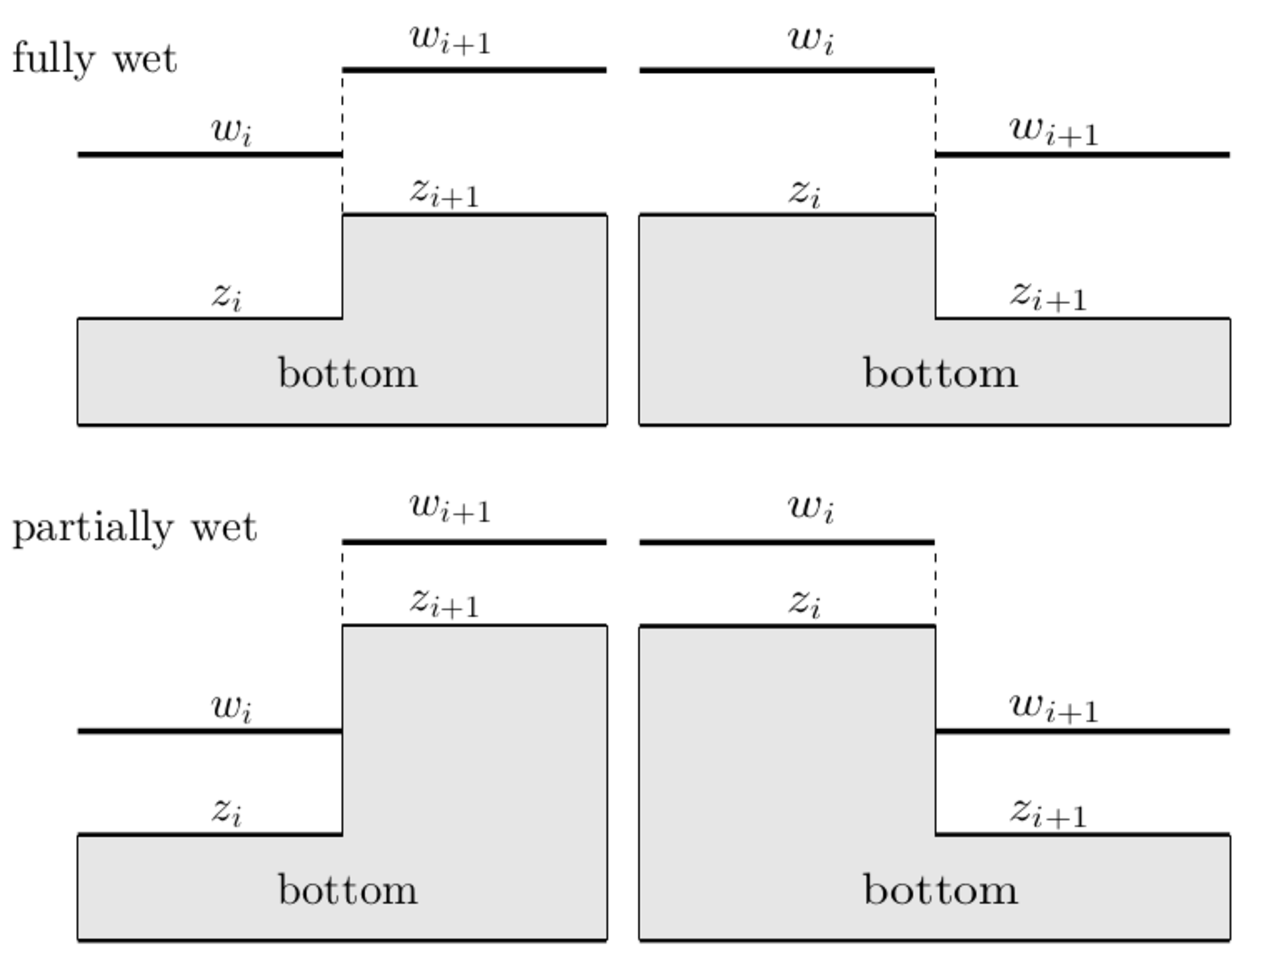
\includegraphics[scale=0.4]{1}
\caption{Examples of interfaces: fully wet (top), and partially wet (bottom).}
\label{fig1}
\end{figure}
After the water heights $h_{i-\frac{1}{2}+}$ and $h_{i+\frac{1}{2}-}$ are reconstructed in the following three HR schemes, the conservative variables are defined as 
\begin{align}
{U_{i + \frac{1}{2} - }}: = \left( {\begin{array}{*{20}{c}}
{{h_{i + \frac{1}{2} - }}}\\
{{h_{i + \frac{1}{2} - }}{u_{i + \frac{1}{2} - }}}
\end{array}} \right), \hspace{2mm} {U_{i - \frac{1}{2} + }}: = \left( {\begin{array}{*{20}{c}}
{{h_{i - \frac{1}{2} + }}}\\
{{h_{i - \frac{1}{2} + }}{u_{i - \frac{1}{2} + }}}
\end{array}} \right) \mbox{ with } {u_{i + \frac{1}{2} - }} = {u_{i - \frac{1}{2} + }} = {u_i}. 
\end{align}

\subsection{The original HR method}
Audusse et al. \cite{Audusse2004} introduce their first order HR scheme by choosing the \textit{intermediate bottom} as 
\begin{align}
\label{3.6}
b_{i + \frac{1}{2}}^{\rm AUD}: = \max \left( {{b_i},{b_{i + 1}}} \right),
\end{align}
and the \textit{interface water height} as 
\begin{align}
\label{3.7}
h_{i + \frac{1}{2} - }^{\rm AUD}: = {\left( {{w_i} - b_{i + \frac{1}{2}}^{\rm AUD}} \right)^ + }, \hspace{2mm} h_{i + \frac{1}{2} + }^{\rm AUD}: = {\left( {{w_{i + 1}} - b_{i + \frac{1}{2}}^{\rm AUD}} \right)^ + }.
\end{align}
The source term is discretized as 
\begin{align}
s_{i + \frac{1}{2} - }^{\rm AUD}: &= \frac{g}{{2\Delta x}}\left( {{{\left( {h_{i + \frac{1}{2} - }^{\rm AUD}} \right)}^2} - h_i^2} \right),\\
s_{i + \frac{1}{2} + }^{\rm AUD}: &= \frac{g}{{2\Delta x}}\left( {h_{i + 1}^2 - {{\left( {h_{i + \frac{1}{2} + }^{\rm AUD}} \right)}^2}} \right).
\end{align}

\subsection{The HR method of Morales et al.}
The HR scheme of Morales et al. \cite{Morales2013} is identical to that of Audusse's scheme,
\begin{align}
b_{i + \frac{1}{2}}^{\rm MOR}: = b_{i + \frac{1}{2}}^{\rm AUD}, \hspace{2mm} h_{i + \frac{1}{2} - }^{\rm MOR}: = h_{i + \frac{1}{2} - }^{\rm AUD}, \hspace{2mm} h_{i + \frac{1}{2} + }^{\rm MOR}: = h_{i + \frac{1}{2} + }^{\rm AUD},
\end{align}
and the source term is defined as
\begin{align}
s_{i + \frac{1}{2} - }^{MOR}: = s_{i + \frac{1}{2} - }^{\rm AUD}, \hspace{2mm} s_{i + \frac{1}{2} + }^{MOR}: = s_{i + \frac{1}{2} + }^{\rm AUD},
\end{align}
except for the partially wet interfaces \eqref{3.4}, where water either flows downhill or flows uphill with enough kinetic energy to climb the jump of the bottom at the interface. This results in the following two cases.
\begin{itemize}
\item \textit{$b_i < b_{i+1}$ (ascending bottom)}. If $u_i <0$, or $u_i >0$ and 
\begin{align}
\label{3.12}
\frac{{{{\left| {{u_i}} \right|}^2}}}{2} + g\left( {{w_i} - {b_{i + 1}}} \right) \ge \frac{3}{2}\sqrt {g{{\left( {{h_i}\left| {{u_i}} \right|} \right)}^3}} ,
\end{align}
then the left interface source term is redefined as 
\begin{align}
s_{i + \frac{1}{2} - }^{\rm MOR}: =  - \frac{g}{{\Delta x}}\frac{{{h_i}}}{2}\left( {b_{i + \frac{1}{2}}^{\rm MOR} - {b_i}} \right).
\end{align}
\item \textit{$b_i > b_{i+1}$ (descending bottom)}. If $u_{i+1} >0$, or $u_{i+1}<0$ and 
\begin{align}
\label{3.14}
\frac{{{{\left| {{u_{i + 1}}} \right|}^2}}}{2} + g\left( {{w_{i + 1}} - {b_i}} \right) \ge \frac{3}{2}\sqrt {g{{\left( {{h_{i + 1}}\left| {{u_{i + 1}}} \right|} \right)}^3}} ,
\end{align} 
then the right interface source term is redefined as 
\begin{align}
s_{i + \frac{1}{2} + }^{\rm MOR}: =  - \frac{g}{{\Delta x}}\frac{{{h_{i + 1}}}}{2}\left( {{b_{i + 1}} - b_{i + \frac{1}{2}}^{\rm MOR}} \right).
\end{align}
\end{itemize}

\subsection{The third HR method}
For the third HR method, the intermediate bottom is defined as
\begin{align}
\label{3.16}
b_{i + \frac{1}{2}}^{\rm CN}: = \min \left( {\max \left( {{b_i},{b_{i + 1}}} \right),\min \left( {{w_i},{w_{i + 1}}} \right)} \right). 
\end{align}
The interface water heights are given by
\begin{align}
\label{3.17}
h_{i + \frac{1}{2} - }^{\rm CN}: = \min \left( {{w_i} - b_{i + \frac{1}{2}}^{\rm CN},{h_i}} \right), \hspace{2mm} h_{i + \frac{1}{2} + }^{\rm CN}: = \min \left( {{w_{i + 1}} - b_{i + \frac{1}{2}}^{\rm CN},{h_{i + 1}}} \right),
\end{align}
and the interface source terms are defined as 
\begin{align}
s_{i + \frac{1}{2} - }^{CN}: &=  - \frac{g}{{\Delta x}}\frac{{{h_i} + h_{i + \frac{1}{2} - }^{CN}}}{2}\left( {b_{i + \frac{1}{2}}^{CN} - {b_i}} \right),\\
s_{i + \frac{1}{2} + }^{CN}: &=  - \frac{g}{{\Delta x}}\frac{{h_{i + \frac{1}{2} + }^{CN} + {h_{i + 1}}}}{2}\left( {{b_{i + 1}} - b_{i + \frac{1}{2}}^{CN}} \right).
\end{align}

\begin{remark}
For fully wet interfaces, all schemes are identical. The differences for the partially wet case are rather subtle.
\end{remark}

\subsection{The numerical flux}
In \cite[p. 763]{Chen2017}, the authors used Harten-Lax-van Leer (HLL)-type Riemann solvers,
\begin{align}
\label{3.20}
{\mathcal{F}_{\rm HLL}}\left( {{U_ - },{U_ + }} \right) = \frac{{{s^ + }F\left( {{U_ - }} \right) - {s^ - }F\left( {{U_ + }} \right) + {s^ + }{s^ - }\left( {{U_ + } - {U_ - }} \right)}}{{{s^ + } - {s^ - }}},
\end{align}
where the smallest and largest wave speed $s^-$ and $s^+$ are chosen as
\begin{align}
\label{3.21}
{s^ - } = \min \left( {{u_ - } - {a_ - },{u_ + } - {a_ + },0} \right), \hspace{2mm} {s^ + } = \max \left( {{u_ - } + {a_ - },{u_ + } + {a_ + },0} \right),
\end{align}
with gravitational wave speed $a = \sqrt {gh}$.

The following inequalities satisfied by the HLL flux are crucial for the stability analysis. The first one states that there is no numerical mass flux out of an empty cell, and is used to prove positivity of the water height later.

\begin{lemma}
The first component of the HLL flux satisfies 
\begin{align}
\label{3.22}
{\mathcal{F}^h}\left( {\left( {0,0} \right),\left( {h,hu} \right)} \right) \le 0, \hspace{2mm} {\mathcal{F}^h}\left( {\left( {h,hu} \right),\left( {0,0} \right)} \right) \ge 0.
\end{align}
\end{lemma}

\begin{proof}
From the definition of the wave speeds \eqref{3.21}, the value of HLL flux at $U_-=\left(0,0\right)$ and $U_+ = \left(h,hu\right)$ is 
\begin{align}
{\mathcal{F}_{\rm HLL}}\left( {\left( {0,0} \right),\left( {h,hu} \right)} \right) = \frac{{ - {s^ - }\left( {hu,h{u^2} + \frac{1}{2}g{h^2}} \right) + {s^ + }{s^ - }\left( {h,hu} \right)}}{{{s^ + } - {s^ - }}}.
\end{align}
Hence, the first component of the HLL flux is given by 
\begin{align}
\mathcal{F}_{HLL}^h\left( {\left( {0,0} \right),\left( {h,hu} \right)} \right) = \frac{{ - {s^ - }hu + {s^ + }{s^ - }h}}{{{s^ + } - {s^ - }}} = h{s^ - }\frac{{{s^ + } - u}}{{{s^ + } - {s^ - }}}.
\end{align}
Since $h\ge 0$, $s^-\le 0$, $s^+ \ge u$, $s^+ >s^-$, the last equality gives us $\mathcal{F}_{HLL}^h \le 0$. 

Similarly,
\begin{align}
{\mathcal{F}_{\rm HLL}}\left( {\left( {h,hu} \right),\left( {0,0} \right)} \right) = \frac{{{s^ + }\left( {hu,h{u^2} + \frac{1}{2}g{h^2}} \right) - {s^ + }{s^ - }\left( {h,hu} \right)}}{{{s^ + } - {s^ - }}},
\end{align}
and thus
\begin{align}
\mathcal{F}_{\rm HLL}^h\left( {\left( {h,hu} \right),\left( {0,0} \right)} \right) = {s^ + }h\frac{{u - {s^ - }}}{{{s^ + } - {s^ - }}}.
\end{align}
Since $h\ge 0$, $s^+\ge 0$, $u\ge s^-$, $s^+ > s^-$, the last equality implies that $\mathcal{F}_{\rm HLL}^h \ge 0$. 
\end{proof}
The second inequality is used to prove the semidiscrete entropy inequality. It states that the numerical mass flux into a vacuum cell is at least as large as the physical mass flux. 

\begin{lemma}
The first component of the HLL flux satisfies
\begin{align}
\mathcal{F}_{\rm HLL}^h\left( {\left( {h,hu} \right),\left( {0,0} \right)} \right) - hu \ge 0, \hspace{2mm} hu - \mathcal{F}_{\rm HLL}^h\left( {\left( {0,0} \right),\left( {h,hu} \right)} \right) \ge 0.
\end{align}
\end{lemma}

\begin{proof}
The proof follows from \eqref{3.20} and \eqref{3.21} via
\begin{align*}
\mathcal{F}_{\rm HLL}^h\left( {\left( {h,hu} \right),\left( {0,0} \right)} \right) - hu &= \frac{{{s^ + }hu - {s^ + }{s^ - }h}}{{{s^ + } - {s^ - }}} - hu =  - \frac{{{s^ - }h\left( {{s^ + } - u} \right)}}{{{s^ + } - {s^ - }}} \ge 0,\\
hu - \mathcal{F}_{\rm HLL}^h\left( {\left( {0,0} \right),\left( {h,hu} \right)} \right) &= hu - \frac{{ - {s^ - }hu + {s^ + }{s^ - }h}}{{{s^ + } - {s^ - }}} = \frac{{{s^ + }h\left( {u - {s^ - }} \right)}}{{{s^ + } - {s^ - }}} \ge 0.
\end{align*}
This completes our proof.
\end{proof}

\subsection{Interpretation via subcell reconstructions}
Recall that in \cite{Chen2017} the \textit{singular layers} (or \textit{internal boundary layers}) are defined by
\begin{align}
\widehat C_{i + \frac{1}{2}}^\varepsilon : = \left[ {{x_{i + \frac{1}{2}}} - \varepsilon ,{x_{i + \frac{1}{2}}} + \varepsilon } \right],\forall i \in \mathcal{E}.
\end{align}
Over each of these infinitesimal layers the bottom is reconstructed continuously by a function $b_\varepsilon \left(x\right)$. The flow variables are reconstructed by piecewise continuous functions $h_\varepsilon \left(x\right)$, $w_\varepsilon \left(x\right)$, and $u_\varepsilon \left(x\right)$ over the singular subcells
\begin{align}
\widehat C_{i + \frac{1}{2} - }^\varepsilon : = \left[ {{x_{i + \frac{1}{2}}} - \varepsilon ,{x_{i + \frac{1}{2}}}} \right] \mbox{ and } \widehat C_{i + \frac{1}{2} + }^\varepsilon : = \left[ {{x_{i + \frac{1}{2}}},{x_{i + \frac{1}{2}}} + \varepsilon } \right], \hspace{2mm} \forall i \in \mathcal{E}.
\end{align}
These reconstructions provide the data of the Riemann problem at the interface, with an approximate Riemann solver $F_\varepsilon \left(x_{i+\frac{1}{2}}\right)$. The source term is computed over the singular subcells. Together, this gives the \textit{residuum}
\begin{align}
R_i^\varepsilon : =  - \frac{1}{{\Delta x}}\left( {{F_\varepsilon }\left( {{x_{i + \frac{1}{2}}}} \right) - {F_\varepsilon }\left( {{x_{i - \frac{1}{2}}}} \right)} \right) + \frac{1}{{\Delta x}}\int_{{C_i}} {S\left( {{U_\varepsilon }\left( x \right),{b_\varepsilon }\left( x \right)} \right)dx} .
\end{align}

\subsubsection{Splitting the cells into subcells}
Let us denote the \textit{interior subcell} by $C_i^\varepsilon : = \left[ {{x_{i - \frac{1}{2}}} + \varepsilon ,{x_{i + \frac{1}{2}}} - \varepsilon } \right]$. Then
\begin{align}
{C_i} = \widehat C_{i - \frac{1}{2} + }^\varepsilon  \cup C_i^\varepsilon  \cup \widehat C_{i + \frac{1}{2} - }^\varepsilon .
\end{align}
The \textit{piecewise continuous reconstruction} is defined as follows.

\begin{definition}[subcell reconstruction] 
\label{def1}
Given values $\varphi _i$ and $\varphi _{i+\frac{1}{2}\pm}$ for $i\in \mathbb{Z}$, let $\widehat \varphi _{i + \frac{1}{2} \pm }^\varepsilon :\widehat C_{i + \frac{1}{2} \pm }^\varepsilon  \to \mathbb{R}$ be Lipschitz continuous functions with boundary values
\begin{align}
{\varphi _{i + \frac{1}{2} \pm }}\left( {{x_{i + \frac{1}{2}}}} \right) = {\varphi _{i + \frac{1}{2} \pm }}, \hspace{2mm} {\varphi _{i + \frac{1}{2} \pm }}\left( {{x_{i + \frac{1}{2}}} \pm \varepsilon } \right) = {\varphi _{i + \frac{{1 \pm 1}}{2}}}.
\end{align}
Then $\varphi _\varepsilon: \mathbb{R}\to \mathbb{R}$ is the piecewise continuous function given by 
\begin{equation*}
{\varphi _\varepsilon }\left( x \right): = \left\{ \begin{split}
{\varphi _i}, \mbox{ if } x \in C_i^\varepsilon ,\\
\widehat \varphi _{i + \frac{1}{2} \pm }^\varepsilon , \mbox{ if } x \in \widehat C_{i + \frac{1}{2} \pm }^\varepsilon .
\end{split} \right.
\end{equation*}
\end{definition}

\begin{remark}
If $\widehat \varphi _{i + \frac{1}{2} - }^\varepsilon$ and $\widehat \varphi _{i + \frac{1}{2} + }^\varepsilon$ are both linear, we call them the \emph{standard subcell reconstruction at interface} $x_{i+\frac{1}{2}}$. The only exception from the standard subcell reconstruction will occur in the definition of the water level for Audusse's and Morales' schemes for partially wet interfaces.
\end{remark}

\subsubsection{Reconstruction of the bottom $b_\varepsilon \left(x\right)$}
For all three HR schemes, a continuous bottom is defined by the standard subcell reconstruction (Def. \ref{def1}) with 
\begin{align}
{b_{i - \frac{1}{2} + }}: = {b_{i - \frac{1}{2}}}, \hspace{2mm} {b_{i + \frac{1}{2} - }}: = {b_{i + \frac{1}{2}}} .
\end{align}
The reconstructed bottom is globally continuous for fixed $\varepsilon >0$, but will have steep layers in $\widehat C_{i + \frac{1}{2} - }^\varepsilon $ and $\widehat C_{i + \frac{1}{2} - }^\varepsilon $.

\subsubsection{Infinitesimal HR}
The water level and height are now reconstructed. Several modern well-balanced schemes, as well as the third HR schemes, use the fact that the water level $w\left(x\right)$ is constant for still water. Thus, the piecewise constant reconstruction becomes exact for this equilibrium state. 

Given the bottom topography $b_\varepsilon \left(x\right)$, these schemes reconstruct the water level $w_\varepsilon \left(x\right)$. The reconstructed water height is then reconstructed simply as 
\begin{align}
{h_\varepsilon }\left( x \right): = {w_\varepsilon }\left( x \right) - {b_\varepsilon }\left( x \right).
\end{align}
The \textit{conservative variables} are given by
\begin{align}
{U_\varepsilon }\left( x \right): = \sum\limits_{i = 1}^{{N_x}} {\left( {\begin{array}{*{20}{c}}
{{h_\varepsilon }\left( x \right)}\\
{{h_\varepsilon }\left( x \right){u_i}}
\end{array}} \right){{\bf 1}_{{C_i}}}\left( x \right)} ,
\end{align}
The following integral averages of $h_\varepsilon \left(x\right)$ in subcells $\widehat C_{i + \frac{1}{2} - }^\varepsilon$ and $\widehat C_{i + \frac{1}{2} + }^\varepsilon $ are used to calculate the flux and the source term later. 
\begin{align}
\label{3.36}
{{\bar h}_{i + \frac{1}{2} - }}: = \frac{1}{\varepsilon }\int_{\widehat C_{i + \frac{1}{2} - }^\varepsilon } {{h_\varepsilon }\left( x \right)dx} , \hspace{2mm} {{\bar h}_{i + \frac{1}{2} + }}: = \frac{1}{\varepsilon }\int_{\widehat C_{i + \frac{1}{2} + }^\varepsilon } {{h_\varepsilon }\left( x \right)dx} .
\end{align}

\paragraph{3.5.3.1. The original HR method.} Define $w_\varepsilon \left(x\right)$ as in Def. \ref{def1}, with 
\begin{align}
w_i^{\rm AUD}: &= {h_i} + {b_i}, \hspace{2mm} w_{i + 1}^{\rm AUD}: = {h_{i + 1}} + {b_{i + 1}},\\
w_{i + \frac{1}{2} - }^{\rm AUD}: &= \max \left( {b_{i + \frac{1}{2}}^{\rm AUD},  \hspace{2mm} {w_i}} \right), \hspace{2mm} w_{i + \frac{1}{2} + }^{\rm AUD}: = \max \left( {b_{i + \frac{1}{2}}^{\rm AUD},{w_{i + 1}}} \right). \label{3.38}
\end{align}
In the fully wet case (see Fig. \ref{fig2}),
\begin{align}
\widehat w_{i + \frac{1}{2} - }^{\rm AUD} \equiv {w_i}, \hspace{2mm} \widehat w_{i + \frac{1}{2} + }^{\rm AUD} \equiv {w_{i + 1}},
\end{align}

\begin{figure}[H]
\centering
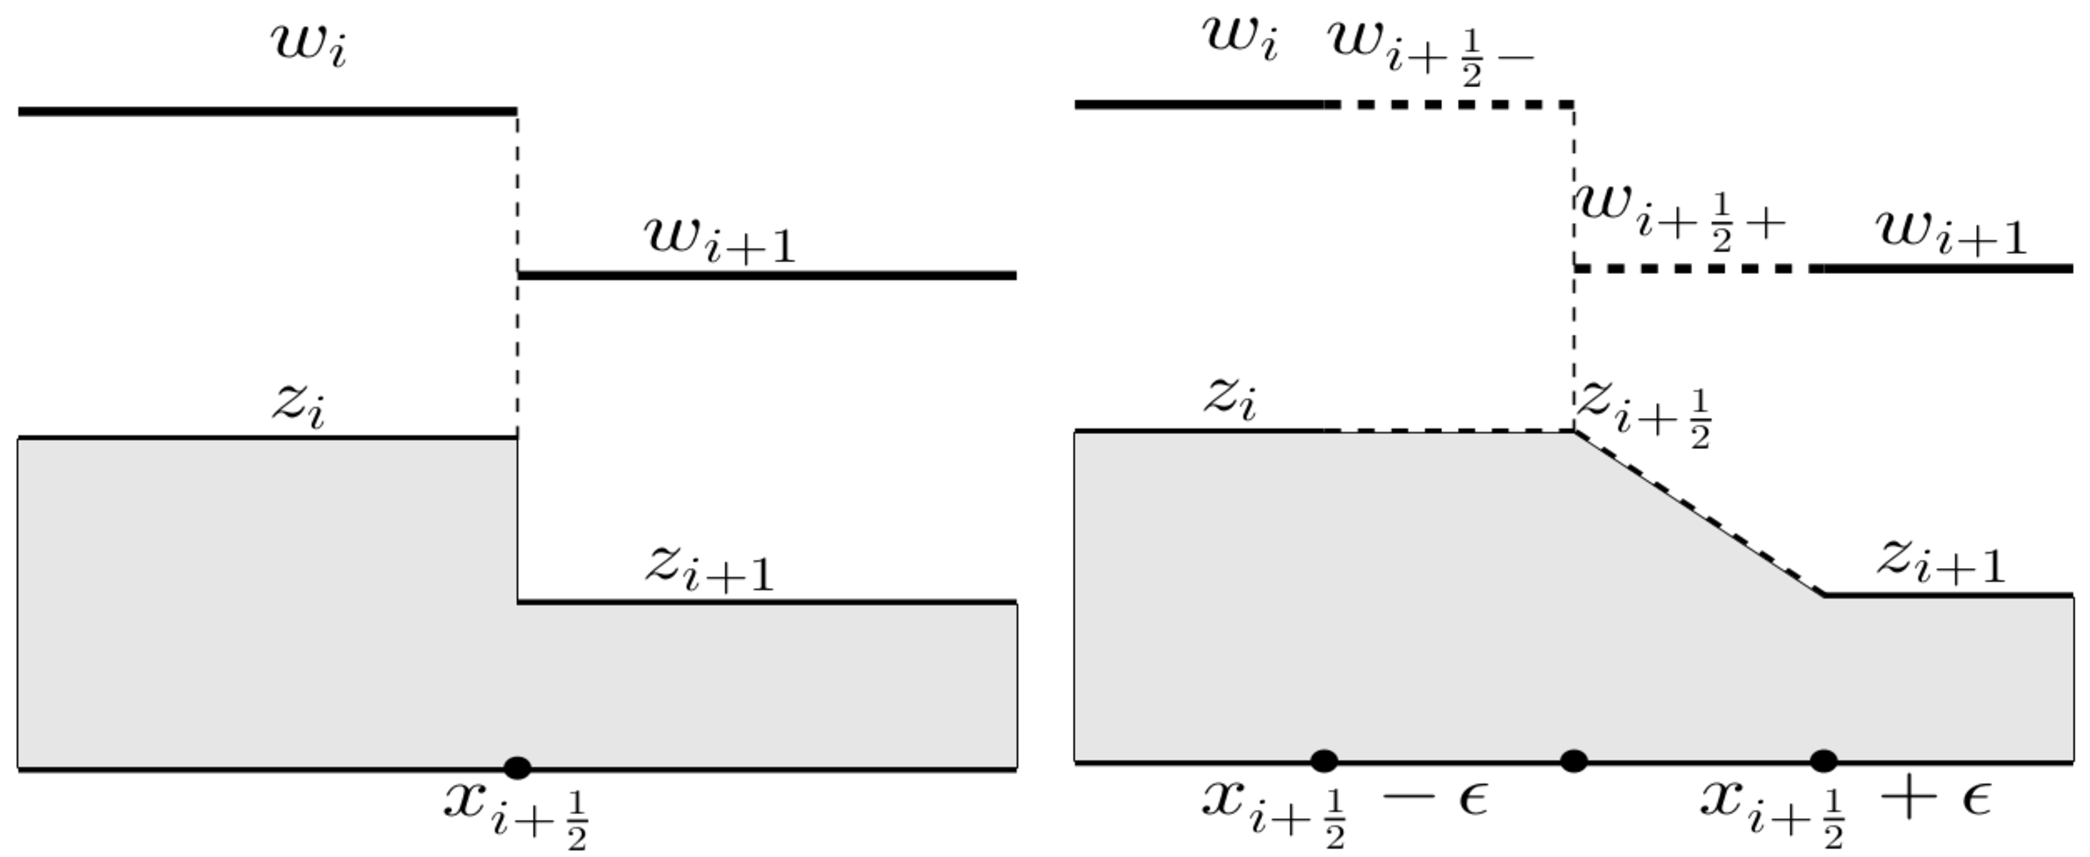
\includegraphics[scale=0.35]{2}
\caption{Subcell reconstruction of topography and water level for the fully wet case. Left: Riemann data. Right: reconstructed $b_\varepsilon\left(x\right)$ and $w_\varepsilon \left(x\right)$ for all three HR schemes.}
\label{fig2}
\end{figure}
while in the partially wet case (see Fig. \ref{fig3}), 
\begin{align}
\widehat w_{i + \frac{1}{2} - }^{\rm AUD}\left( x \right): = \max \left( {b_\varepsilon ^{\rm AUD}\left( x \right),{w_i}} \right), \hspace{2mm} \widehat w_{i + \frac{1}{2} + }^{\rm AUD}\left( x \right): = \max \left( {b_\varepsilon ^{\rm AUD}\left( x \right),{w_{i + 1}}} \right).
\end{align}
\begin{figure}[H]
\centering
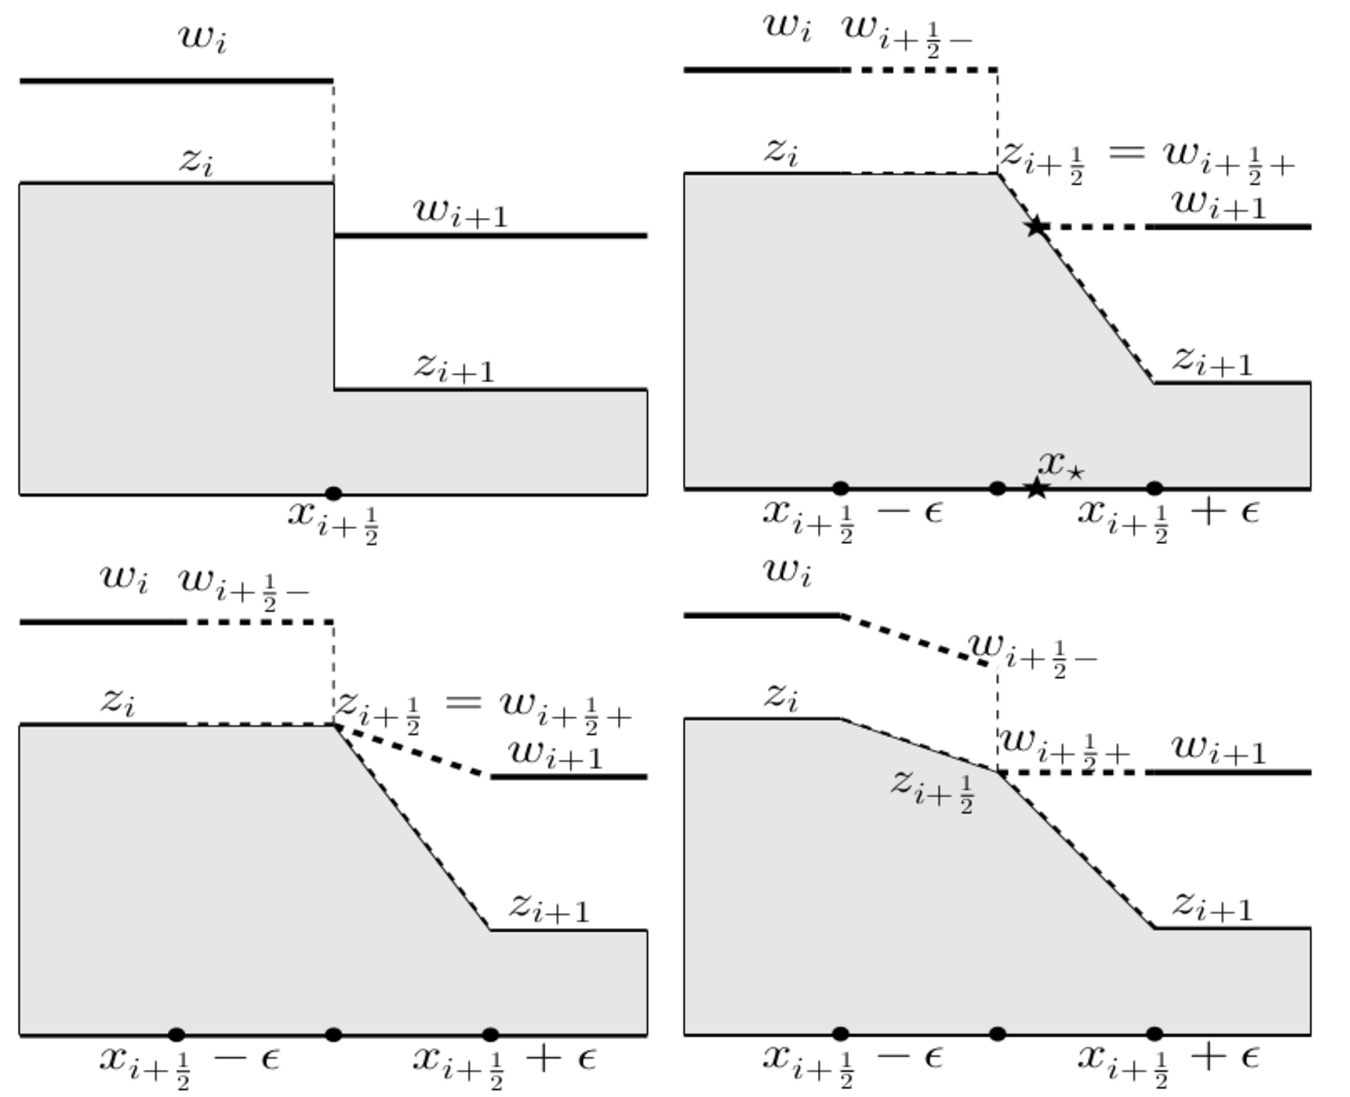
\includegraphics[scale=0.5]{3}
\caption{Subcell reconstruction of topography and water level for the partially wet case. Top left: Riemann data. Top right: Audusse or Morales scheme for slow uphill flow (the vacuum region $\left[x_{i+\frac{1}{2}},x_\star \right]$). Bottom left: Morales scheme for fast uphill flow. Bottom right: CN scheme.}
\label{fig3}
\end{figure}
This is the only instance where the subcell reconstruction may differ from the standard definition. This will happen if and only if the wet-dry front is contained in one of the cells $\widehat C_{i + \frac{1}{2} - }^\varepsilon$ or $\widehat C_{i + \frac{1}{2} - }^\varepsilon$. 

The average of $h_\varepsilon ^{\rm AUD} \left(x\right)$ over subcell $\widehat C_{i + \frac{1}{2} - }^\varepsilon$ is defined as follows (that over subcell $\widehat C_{i + \frac{1}{2} + }^\varepsilon $ is defined similarly). There are two cases to be discussed.
\begin{itemize}
\item[i)] In the fully wet case (in which all three schemes coincide) the water height $\widehat h_{i + \frac{1}{2} + }^{\rm AUD}$ is linear, so 
\begin{align}
\label{3.41}
\bar h_{i + \frac{1}{2} + }^{\rm AUD} = \frac{{h_{i + \frac{1}{2} + }^{\rm AUD} + {h_{i + 1}}}}{2}.
\end{align}
\item[ii)] In the partially wet case, $h_{i + \frac{1}{2} + }^{\rm AUD} = 0$ (see top right of Fig. \ref{fig3}). Assume that the wet front is located at ${x_\star} \in \widehat C_{i + \frac{1}{2} + }^\varepsilon$. Then the average water height is 
\begin{align}
\label{3.42}
\bar h_{i + \frac{1}{2} + }^{\rm AUD} = \frac{{{x_{i + \frac{1}{2}}} + \varepsilon  - {x_*}}}{\varepsilon }\frac{{h\left( {{x_\star}} \right) + {h_{i + 1}}}}{2} = \frac{{{h_{i + 1}}}}{{{b_{i + \frac{1}{2}}} - {b_{i + 1}}}}\frac{{{h_{i + 1}}}}{2},
\end{align}
where we have used the intercept theorem in the last inequality. 
\end{itemize}
Summarizing \eqref{3.41} and \eqref{3.42}, we obtain
\begin{equation}
\label{3.43}
\bar h_{i + \frac{1}{2} + }^{\rm AUD} = \left\{ \begin{split}
& \frac{{{h_{i + 1}} + h_{i + \frac{1}{2} + }^{\rm AUD}}}{2}, & \mbox{ if }h_{i + \frac{1}{2} + }^{\rm AUD} > 0,\\
& \frac{{{h_{i + 1}}}}{2}\frac{{{h_{i + 1}}}}{{b_{i + \frac{1}{2}}^{\rm AUD} - {b_{i + 1}}}}, & \mbox{ if } h_{i + \frac{1}{2} + }^{\rm AUD} = 0.
\end{split} \right.
\end{equation}
Similarly,
\begin{equation}
\label{3.44}
\bar h_{i + \frac{1}{2} - }^{\rm AUD} = \left\{ \begin{split}
& \frac{{{h_i} + h_{i + \frac{1}{2} - }^{\rm AUD}}}{2}, & \mbox{ if } h_{i + \frac{1}{2} - }^{\rm AUD} > 0,\\
& \frac{{{h_i}}}{2}\frac{{{h_i}}}{{b_{i + \frac{1}{2}}^{\rm AUD} - {b_i}}}, & \mbox{ if } h_{i + \frac{1}{2} - }^{\rm AUD} = 0.
\end{split} \right.
\end{equation}

\paragraph{3.5.3.2. The HR scheme of Morales et al.} The continuous bottom of Morales' scheme coincides with that of the original HR scheme: 
\begin{align}
b_\varepsilon ^{\rm MOR}\left( x \right) \equiv b_\varepsilon ^{\rm AUD}\left( x \right).
\end{align}
The water level coincides with that of the original scheme, except for the partially wet interface \eqref{3.4}. If the water flows downhill, or uphill with enough kinetic energy to climb the discrete jump of the bottom, i.e., \eqref{3.12} (resp., \eqref{3.14}) holds, then over ${\widehat C_{i + \frac{1}{2} - }}$ (resp. ${\widehat C_{i + \frac{1}{2} + }}$) the reconstructed water level $w_\varepsilon ^{\rm MOR} \left(x\right)$ is given by the standard subcell reconstruction (see Def. \ref{def1}) instead of Audusse's piecewise linear reconstruction \eqref{3.38} (see Fig. \ref{fig3}). Then the local averages of $h_\varepsilon ^{\rm MOR}\left(x\right)$ over subcells $\widehat C_{i + \frac{1}{2} - }^\varepsilon$ (resp., $\widehat C_{i + \frac{1}{2} + }^\varepsilon $) are simply
\begin{align}
\label{3.46}
\bar h_{i + \frac{1}{2} - }^{\rm MOR} = \frac{{{h_i} + h_{i + \frac{1}{2} - }^{\rm MOR}}}{2} = \frac{{{h_i}}}{2}, \hspace{2mm} \bar h_{i + \frac{1}{2} + }^{\rm MOR} = \frac{{{h_{i + 1}} + h_{i + \frac{1}{2} + }^{\rm MOR}}}{2} = \frac{{{h_{i + 1}}}}{2},
\end{align}
since ${h_{i + \frac{1}{2} - }^{MOR}} =0$ (resp., ${h_{i + \frac{1}{2} +}^{MOR}} =0$).

\paragraph{3.5.3.3. The third HR scheme.} The continuous bottom of the third HR scheme in \cite{Chen2017}, denoted by $b_\varepsilon ^{\rm CN}$ is defined by the standard subcell reconstruction with 
\begin{align}
b_{i + \frac{1}{2} - }^{\rm CN} = b_{i + \frac{1}{2} + }^{\rm CN} = b_{i + \frac{1}{2}}^{\rm CN} .
\end{align}
The reference values for the water surface are given by
\begin{align}
w_{i + \frac{1}{2} - }^{\rm CN}: = \min \left( {{w_i},b_{i + \frac{1}{2}}^{\rm CN} + {h_i}} \right),\hspace{2mm} w_{i + \frac{1}{2} + }^{\rm CN}: = \min \left( {{w_{i + 1}},b_{i + \frac{1}{2}}^{\rm CN} + {h_{i + 1}}} \right),
\end{align}
and the reference values for the water depth are given by \eqref{3.17}. Due to the linearity of ${\widehat h_{i + \frac{1}{2} - }}$ (resp., ${\widehat h_{i + \frac{1}{2} + }}$), the average values of $h_\varepsilon$ over the singular subcells $\widehat C_{i + \frac{1}{2} - }^\varepsilon $ (resp., $\widehat C_{i + \frac{1}{2} + }^\varepsilon$) are
\begin{align}
\label{3.49}
\bar h_{i + \frac{1}{2} - }^{\rm CN} = \frac{{{h_i} + h_{i + \frac{1}{2} - }^{\rm CN}}}{2}, \hspace{2mm} \bar h_{i + \frac{1}{2} + }^{\rm CN} = \frac{{{h_i} + h_{i + \frac{1}{2} + }^{\rm CN}}}{2}.
\end{align}

\begin{remark}
From \eqref{3.43}, \eqref{3.44}, \eqref{3.46} and \eqref{3.49}, the subcell averages ${{\bar h}_{i + \frac{1}{2} - }}$ and ${{\bar h}_{i + \frac{1}{2} + }}$ of $h_\varepsilon \left(x\right)$ over subcells $\widehat C_{i + \frac{1}{2} - }^\varepsilon $ and $\widehat C_{i + \frac{1}{2} + }^\varepsilon $ obtained by the three schemes are in fact independent of $\varepsilon$.
\end{remark}

\begin{proof}
. . . . . 
\end{proof}

\subsubsection{Fluxes and source terms based on subcell reconstructions}
For all three hydrostatic schemes the flux vector $F_\varepsilon \left(x\right)$ is reconstructed by the standard subcell reconstruction (see Def. \ref{def1}) with reference values
\begin{align}
\label{3.50}
{F_i}: = F\left( {{U_i}} \right), \hspace{2mm} {F_{i + \frac{1}{2} - }}: = {F_{i + \frac{1}{2} + }}: = {F_{i + \frac{1}{2}}},
\end{align}
where
\begin{align}
{F_{i + \frac{1}{2}}}: = \mathcal{F}_{\rm HLL} \left( {{U_{i + \frac{1}{2} - }},{U_{i + \frac{1}{2} + }}} \right)
\end{align}
is an approximate Riemann solver. Note that $F_\varepsilon \left(x\right)$ is globally continuous. The definition of the reconstructed source term $S_\varepsilon \left(x\right) := \left(0,s_\varepsilon \left(x\right)\right)^T$ takes the natural form
\begin{align}
\label{3.52}
{s_\varepsilon }\left( x \right): =  - g{h_\varepsilon }\left( x \right){b_\varepsilon }'\left( x \right),
\end{align}
and hence corresponds directly to \eqref{1.4}.

Given \eqref{3.50}-\eqref{3.52}, we now introduce the reconstructed, cell-averaged residuum by
\begin{align}
R_i^\varepsilon : =  - \frac{1}{{\Delta x}}\left( {{F_\varepsilon }\left( {{x_{i + \frac{1}{2}}}} \right) - {F_\varepsilon }\left( {{x_{i - \frac{1}{2}}}} \right)} \right) + \frac{1}{{\Delta x}}\int_{{C_i}} {S\left( {{U_\varepsilon }\left( x \right),{b_\varepsilon }\left( x \right)} \right)dx} .
\end{align}
Depending on the choice of hydrostatic scheme, we denote the residuum by $R_i^{\varepsilon ,\rm AUD}$, $R_i^{\varepsilon ,\rm MOR}$, and $R_i^{\varepsilon ,\rm CN}$.

\begin{theorem}
For each of the three hydrostatic schemes, and for each cell $C_i$, the reconstructed residuums are independent of $\varepsilon$, $R_i^\varepsilon  = {{\bar R}_i}$ for all $\varepsilon >0$, and coincide with the original definitions given above:
\begin{align}
\bar R_i^{\rm AUD} = R_i^{\rm AUD},\bar R_i^{\rm MOR} = R_i^{\rm MOR},\bar R_i^{\rm CN} = R_i^{\rm CN}.
\end{align}
\end{theorem}

\begin{proof}
See \cite[pp. 768--769]{Chen2017}
\end{proof}

\begin{remark}
The main advantage of the third HR scheme is its accuracy for shallow downhill flows. . . . . 
\end{remark}

\subsection{Comparison of the HR schemes}
The third HR scheme only differs from the previous methods in the partially wet case \eqref{3.4}. Additionally, it differs only in $\bar h _{i+\frac{1}{2}\pm}$ and $b_{i+\frac{1}{2}}$.

\begin{prop}
\begin{itemize}
\item[i)] For all interfaces $x_{i+\frac{1}{2}}$,
\begin{align}
h_{i + \frac{1}{2} \pm }^{\rm AUD} = h_{i + \frac{1}{2} \pm }^{\rm MOR} = h_{i + \frac{1}{2} \pm }^{\rm CN}
\end{align}
and 
\begin{align}
0 \le {h_{i + \frac{1}{2} - }} \le {h_i},\hspace{2mm} 0 \le {h_{i + \frac{1}{2} + }} \le {h_{i + 1}}.
\end{align}
\item[ii)] For fully wet interfaces $x_{i+\frac{1}{2}}$,
\begin{align}
b_{i + \frac{1}{2}}^{\rm AUD} = b_{i + \frac{1}{2}}^{\rm MOR} = b_{i + \frac{1}{2}}^{\rm CN} \mbox{ and } \bar h_{i + \frac{1}{2} \pm }^{\rm AUD} = \bar h_{i + \frac{1}{2} \pm }^{\rm MOR} = \bar h_{i + \frac{1}{2} \pm }^{\rm CN}.
\end{align}
\item[iii)] For partially wet interfaces $x_{i+\frac{1}{2}}$ (see \eqref{3.4}), and if water flows downhill, or if it flows uphill with too little kinetic energy to climb the discrete jump of the bottom (i.e., neither \eqref{3.12} nor \eqref{3.14} holds), then
\begin{align}
b_{i + \frac{1}{2}}^{\rm AUD} = b_{i + \frac{1}{2}}^{\rm MOR} \mbox{ and } \bar h_{i + \frac{1}{2} \pm }^{\rm AUD} = \bar h_{i + \frac{1}{2} \pm }^{\rm MOR}.
\end{align}
\end{itemize}
\end{prop}

\begin{proof}
The proof is a direct computation based on the definition of the interface values \eqref{3.6}, \eqref{3.7}, \eqref{3.16}, and \eqref{3.17}, and the integral averages of the subcell water heights defined in \eqref{3.36}.

. . . . . 
\end{proof}

\subsection{Stability analysis}
Recall that the well-known convex decomposition of the semidiscrete finite volume scheme \eqref{1.3} is defined by
\begin{align}
\frac{d}{{dt}}{U_i}\left( t \right) &= {R_{i - \frac{1}{2} + }} + {R_{i - \frac{1}{2} + }}\\
: &=  - \frac{1}{{\Delta x}}\left( {F\left( {{U_i}} \right) - {F_{i - \frac{1}{2}}}} \right) + {S_{i - \frac{1}{2} + }} - \frac{1}{{\Delta x}}\left( {{F_{i + \frac{1}{2}}} - F\left( {{U_i}} \right)} \right) + {S_{i + \frac{1}{2} - }}.
\end{align}
The following theorem states that the third HR scheme preserves the positivity of the water height under the same condition as Audusse's scheme.

\begin{theorem}[Positivity of water height] 
Under condition \eqref{3.22}, the new semidiscrete HR scheme guarantees nonnegative water height for the homogeneous shallow water equations.
\end{theorem}

\begin{proof}
. . . . .
\end{proof}
Before proving that the third HR scheme is well-balanced, we would like to distinguish the follow two classes of equilibria.

\begin{definition}
\label{def2}
\begin{itemize}
\item[i)] Given a constant water level $w_{eq}$, the \emph{still water equilibrium} is given by $u\left(x\right) \equiv 0$ and 
\begin{align}
h\left( x \right) + b\left( x \right) \equiv {w_{eq}}.
\end{align}
The cell averages are consistent with the still water equilibrium, if for all $i$, $u_i = 0$ and 
\begin{align}
h_i + b_i = w_{eq}.
\end{align}
\item[ii)] The \emph{lake at rest equilibrium} is given by $u\left(x\right) \equiv 0$ and 
\begin{align}
h\left( x \right){\partial _x}\left( {h\left( x \right) + b\left( x \right)} \right) \equiv 0,
\end{align}
for some constant $w_{eq} \ge \max _{x\in \mathbb{R}} b\left(x\right)$. Moreover, near a wet-dry interface, the dry part of $b$ should not be lower than the adjacent water level.

The cell averages are \emph{locally} (at interface $x_{i+\frac{1}{2}}$) \emph{consistent with the lake at rest}, if $u_i = u_{i+1}=0$ and either $x_{i+\frac{1}{2}}$ is an interior interface (the still water case)
\begin{align}
{h_i} > 0,{h_{i + 1}} > 0, \mbox{ and } {h_i} + {b_i} = {h_{i + 1}} + {b_{i + 1}},
\end{align}
or a dry-wet front
\begin{align}
{h_i} = 0,{h_{i + 1}} > 0, \mbox{ and } {b_i} \ge {h_{i + 1}} + {b_{i + 1}},
\end{align} 
or a wet-dry front
\begin{align}
{h_i} > 0,{h_{i + 1}} = 0, \mbox{ and } {b_{i + 1}} \ge {h_i} + {b_i},
\end{align}
or dry
\begin{align}
h_i = h_{i+1} = 0.
\end{align}
The cell averages are \emph{globally consistent with the lake at rest}, if they are locally consistent with the lake at rest for all interfaces $x_{i+\frac{1}{2}}$.
\item[iii)] Suppose that the cell averages of the semidiscrete finite volume scheme \eqref{1.3} are consistent with a given equilibrium state. Then we call the scheme \emph{well balanced} for this equilibrium state if $R_i =0$ for all $i$. 
\end{itemize}
\end{definition}

\begin{theorem}[Well-balancing]
The present HR scheme is well-balanced for the lake at rest.
\end{theorem}

\begin{proof}
. . . . .
\end{proof}











% ----------------------------------------------
\section{Offset equilibrium schemes}
It suffices to modify in the upwind decenter scheme \eqref{6} only the discretization of velocity (unlike collocated schemes). 

In \cite{Doyen2014}, the author proposed the following modification:
\begin{align*}
\bar h_{i + \frac{1}{2}}^{n + 1}u_{i + \frac{1}{2}}^{n + 1} = \bar h_{i + \frac{1}{2}}^nu_{i + \frac{1}{2}}^n - \frac{{\Delta t}}{{\Delta x}}\left[ {G_{i + 1}^n - G_i^n + \frac{g}{2}\left( {{{\left( {h_{i + 1}^n} \right)}^2} - {{\left( {h_i^n} \right)}^2}} \right) + \frac{g}{2}\left( {h_i^n + h_{i + 1}^n} \right)\left( {{b_{i + 1}} - {b_i}} \right)} \right],
\end{align*}
which can be rewritten as
\begin{align}
\label{3.1}
\bar h_{i + \frac{1}{2}}^{n + 1}u_{i + \frac{1}{2}}^{n + 1} = \bar h_{i + \frac{1}{2}}^nu_{i + \frac{1}{2}}^n - \frac{{\Delta t}}{{\Delta x}}\left[ {G_{i + 1}^n - G_i^n + \frac{g}{2}\left( {h_i^n + h_{i + 1}^n} \right)\left( {\left( {h_{i + 1}^n + {b_{i + 1}}} \right) - \left( {h_i^n + {b_i}} \right)} \right)} \right].
\end{align}
We can easily verify that this numerical scheme preserves the balance-type states \textit{still water}. 

\begin{prop}[Well-balanced property]
The numerical scheme \eqref{6}-\eqref{3.1} preserved the steady states at rest stated in Proposition \ref{prop4}. 
\end{prop}

\begin{proof}
Suppose that $u_{i+\frac{1}{2}}^n = 0$ and $h_i^n + b_i = \mbox{const}$ for all $i \in \mathcal{E}$, as the proof of Proposition \ref{prop4}, we arrive at 
\begin{align*}
h_i^{n + 1} &= h_i^n, \hspace{2mm} \forall i \in \mathcal{M},\\
\frac{{h_i^n + h_{i + 1}^n}}{2}u_{i + \frac{1}{2}}^{n + 1} &=  - \frac{{\Delta t}}{{\Delta x}}\frac{g}{2}\left( {h_i^n + h_{i + 1}^n} \right)\left( {\left( {h_{i + 1}^n + {b_{i + 1}}} \right) - \left( {h_i^n + {b_i}} \right)} \right), \hspace{2mm} \forall i \in {\mathcal{E}_{\rm int }}.
\end{align*}
It is straightforward to obtain $h_i^{n+1} + b_i =\mbox{const}$ and $u_{i+\frac{1}{2}}^{n+1} =0 $ for all $i \in \mathcal{M}$. 
\end{proof}
In the case where the computational domain includes transitions between zones dry and wet areas, we can draw inspiration from the scheme developed in \cite{Chen2017}.

We define
\begin{equation}
\left\{ \begin{split}
w_i^n &= h_i^n + {b_i},\\
b_{i + \frac{1}{2}}^n &= \min \left( {\max \left( {{b_i},{b_{i + 1}}} \right),\min \left( {w_i^n,w_{i + 1}^n} \right)} \right),\\
h_{i + \frac{1}{2} - }^n &= \min \left( {w_i^n - b_{i + \frac{1}{2}}^n,h_i^n} \right),\\
h_{i + \frac{1}{2} + }^n &= \min \left( {w_{i + 1}^n - b_{i + \frac{1}{2}}^n,h_{i + 1}^n} \right),
\end{split} \right.
\end{equation}
from which we deduce the discretization of the equation in velocity
\begin{align}
\bar h_{i + \frac{1}{2}}^{n + 1}u_{i + \frac{1}{2}}^{n + 1} = \bar h_{i + \frac{1}{2}}^nu_{i + \frac{1}{2}}^n - \frac{{\Delta t}}{{\Delta x}}\left[ {G_{i + 1}^n - G_i^n + \frac{g}{2}\left( {h_i^n + h_{i + 1}^n} \right)\left( {h_{i + \frac{1}{2} + }^n - h_{i + \frac{1}{2} - }^n} \right)} \right].
\end{align}
We can check that this new scheme preserves the steady states of \textit{the lake at rest}. We can assimilate the calculations of water depths $h_{i+\frac{1}{2}\pm}^n$ to a local \textit{runup} algorithm. It remains to be seen whether this scheme practice on unsteady cases.

\printbibliography
%\bibliographystyle{siam}
%\bibliography{MYBIB}
%\Addresses
\end{document}